%===============================================================================
% Autoři: Michal Bidlo, Bohuslav Křena, Jaroslav Dytrych, Petr Veigend a Adam Herout 2018

\chapter{Úvod}

V súčastnosti je zaznamenávanie zvuku už takmer samozrejmosťou pre každé moderné zariadenie určené pre každodenné použitie. Patria medzi nich aj mobilné telefóny a tablety, ktoré sú vybavené zabudovanými mikrofónmi umožňujúcimi bezproblémové nahrávanie zvuku kedykoľvek a kdekoľvek. Na trhu s mobilnými aplikáciami existuje mnoho variácií aplikácií poskytujúcich nahrávanie audia a štandardne už aj výrobca zahŕňa do operačného systému zjednodušenú aplikáciu určenú na nahrávanie. Tieto aplikácie poskytujú prevažne možnosti pre nahrávanie audia nižšej kvality kvôli rapídne rýchlo zväčšujúcemu sa objemu súboru s nahrávkou pri bezstratovom nahrávaní vo vysokej kvalite a primárne dominuje použitie lokálneho úložiska. To však nepokrýva špecifické potreby nahrávania audia, ponúka iba minimálnu konfiguráciu a nepodáva užívateľovi podrobný prehľad o nahrávaní.

Aj tieto problémy rieši táto práca, ktorej cieľom je vytvorenie mobilnej aplikácie pre mobilný operačný systém Android, ktorá je schopná dlhodobého a spoľahlivého nahrávania prostredníctvom interného alebo externého mikrofónu. Súčasťou je aj jednoduchý server, na ktorý sú záznamy počas nahrávania odosielané. Aplikácia je vyvinutá špecificky pre účely výskumu vedúceho tejto práce, pána Ing. Igora Szőkeho, Ph.D. Výskum sa zaoberá meraním impulzných charakteristík miestností.

Obsah práce je rozdelený do logických kapitol, ktoré bližšie vysvetľujú a popisujú princípy a postupy použité pri vytváraní aplikácie. Popis fungovania procesov v aplikácii, spojitosť medzi funkcionalitou a požiadavkami výskumu sú popísané v kapitole~\ref{description}. Táto kapitola podrobne vysvetľuje účel práce a postupy, ktoré sú nezávislé na platforme vývoja a sprostredkúvajú funkcionalitu. V kapitole~\ref{nahravanie} sa nachádza teoretický základ popisujúci digitalizáciu zvuku a atribúty, ktoré ovplyvňujú vlastnosti audia.

Informácie špecifické pre vývoj na Androide, ako napríklad možnosti a obmedzenia nahrávania alebo štruktúra projektu sú popísané v kapitole~\ref{development_android}. Následná implementácia je predmetom kapitoly~\ref{implementace}. Aplikácia používa sieťovú architektúru typu klient-server, takže kapitola popisuje implementačné detaily oboch častí a zahŕňa aj testovanie. Zhodnotenie práce, konečného stavu a potenciálne smery ďalšieho vývoja sú popísané v záverečnej kapitole~\ref{finale}.

\chapter{Formálny a neformálny popis}
\label{description}
\section{Neformálny popis}

Keďže aplikácia, ktorá je predmetom tejto práce je vyvinutá na mieru pre účely výskumu, jej vlastnosti a funkcionalita sú priamo prepojené so zameraním a potrebami tohto výskumu. Nie je určená pre vydanie do obchodu s aplikáciami pre širokú verejnosť a od toho sa odvíja skutočnosť, že na funkcionalitu bol kladený najväčší dôraz, avšak vizuálne prevedenie aplikácie nie je až tak relevantné v tomto prípade použitia. Aplikácia najviac predpokladá existenciu servera, na ktorý sa snaží počas nahrávania pripojiť. Beh aplikácie bez prítomnosti servera je možný, avšak hlavný prípad jej použitia zahŕňa komunikáciu aplikácie so serverom a vzdialené ukladanie.

Použitie pre aplikáciu v rámci výskumu predstavuje médium, pomocou ktorého sa budú vyhotovovať dlhodobé záznamy zvuku s využitím viacerých zariadení s rôznymi verziami operačného systému Android. Nahrávanie môže prebiehať cez mikrofón, ktorý môže byť zabudovaný, fyzicky pripojený do zariadenia cez kábel alebo spojený so zariadením prostredníctvom technológie Bluetooth. Pre zjednodušenie, externý typ mikrofónu bude v texte práce označovať mikrofón pripojený bezdrôtovo a interný bude označovať zabudovaný alebo káblom pripojený mikrofón. Nie sú stanovené žiadne predpoklady na stabilitu a stálosť internetového pripojenia, ktoré je dôležité pre spojenie a komunikáciu so serverom, takže aplikácia musí byť schopná riešiť situácie, kedy nastane problém s internetovým pripojením a zamedziť akémukoľvek negatívnemu dopadu na nahrávku. 

Charakter zvuku, ktorý sa bude nahrávať bude rôzny, často to však bude rečová databáza, ktorá bude prehrávaná v miestnosti pomocou reproduktora. Parametre nahrávania musia byť konfigurovateľné, aby nahrávanie mohlo prebiehať s rozličnými nastaveniami vzorkovacej frekvencie alebo zvukových kanálov. Pri vyhotovovaní veľkého množstva záznamov je dôležitý aj prehľad o jednotlivých nahrávkach, preto je možné každé nahrávanie odlíšiť alebo pridať k nemu manuálne vlastné informačné správy. Vždy by malo byť jasné čo sa v aplikácii práve deje a preto sa na zariadení aj serveri ukladajú informácie o každej podstatnej udalosti, ktorá nastane. Informácie o udalostiach tvoria logovacie súbory, ktoré vznikajú pre každé nahrávanie a obsahujú časovo zoradené udalosti o odosielaní, komunikácii so serverom a poprípade chyby, ktoré nastali.

Predpoklad veľkého množstva súbežných nahrávaní vyžaduje aj spôsob, ako poskytnúť rýchly prehľad o nahrávaniach. Túto funkcionalitu poskytuje práve server, ktorý obsahuje zoznam nahrávaní a prehľadne zobrazuje informácie o ich aktivite, logovacie súbory z nahrávania a aj možnosť stiahnutia posledného nahraného segmentu pre overenie korektnosti nahrávania. Prostredníctvom tohto prehľadu sa dá veľmi rýchlo identifikovať zariadenie, ktoré prestalo so serverom komunikovať alebo iné chyby.

Nahrávané audio musí byť čo najviac zrkadlovým obrazom analógového audia a preto sa nepoužíva nijaká kompresia a nahrávky sa ukladajú vo formáte RAW, ktorý predstavuje nespracované dáta zachytené senzorom. Tento formát sa nedá prehrať na bežných prehrávačoch, pretože neobsahuje hlavičku s údajmi o parametroch o zvuku. Na účely výskumu je však vhodný, pretože audio je v čo najviac pôvodnej forme a parametre, pomocou ktorých sa dá prehrať v špeciálnych prehrávačoch sú vždy zahrnuté v logovacom súbore pre každé nahrávanie, takže konfigurácia sa môže ľubovoľne meniť bez potreby externého ukladania parametrov.

\section{Formálny popis}

V nasledujúcej časti budú popísané základné princípy fungovania aplikácie prostredníctvom popisov postupnosti procesov, procedúr a protokolu, ktorým komunikuje aplikácia so serverom. Toto fungovanie sa nijako neviaže na platformu aplikácie a odvíja sa čisto na základe požiadaviek, ktoré sú na ňu kladené. 

Každé nové nahrávanie predstavuje novú \textbf{session} (sedenie) s jedinečným identifikátorom, v rámci ktorej sú odosielané dáta. Zvuk zo zdroja sa periodicky sníma vo forme vzoriek do buffru. Naplnený buffer tvorí \textbf{segment} (časť nahrávky). Veľkosť segmentov, ktoré sa po sieti odosielajú je nastaviteľná v rámci aplikácie. Odoslané segmenty sa po príchode na server spájajú a tvoria výslednú nahrávku.


\subsection{Protokol}
\label{protokol}

Komunikácia medzi klientom (aplikácia) a serverom funguje prostredníctvom protokolu HTTP, s použitím metódy POST. Pri type použitej metódy je zohľadnená nutnosť prenosu potenciálne veľkého objemu dát (veľkosť segmentu audia je konfigurovateľná), ktorý sa odošle jednorazovo a hodnoty požiadavky sa nikam neukladajú, ani nepotrebujú byť viditeľné. Pri započatí nahrávania vzniká session a jej identifikátor, ktorý sa odosiela v rámci každej požiadavky, aby server vedel z akého zdroja požiadavka smeruje a poskytoval obsluhu viacero súbežných sessions. Server vždy len odpovedá, nikdy sám požiadavku neodosiela. Klient môže pomocou protokolu odoslať:
\begin{itemize}
\item{úvodnú požiadavku nesúcu len typ správy a identifikátor session (handshake),}
\item{záznam do logu (požiadavka nesie identifikátor session, typ požiadavky, časový údaj a správu),}
\item{segment nahrávky (požiadavka nesie identifikátor session, typ požiadavky, počet odosielaných bytov, segment ako reťazec zakódovaný pomocou base64),}
\item{vlastnú správu (požiadavka sa uloží s osobitným označením do logu, môže slúžiť pre označenie istého časového bodu alebo zaznamenanie informácie o nahrávaní),}
\item{ukončujúcu požiadavku zahŕňajúci obsah klientského logu (goodbye).}
\end{itemize}

Príklad výmeny informácie medzi klientom a serverom je znázornený na obrázku~\ref{protocol-example}. Na každú požiadavku sa čaká na odpoveď, ktorá môže značiť bezproblémové prijatie alebo chybu. Ak nastane chyba pri odosielaní úvodnej požiadavky, aplikácia požiadavku ihneď neopakuje, ale v rámci nahrávania sa periodicky snaží vytvoriť spojenie so serverom pomocou tejto úvodnej požiadavky, pretože nemôže bez ustanovenia spojenia so serverom odosielať jednotlivé segmenty. Ak sa neodošle správne záznam do logu, pokus sa už neopakuje. Pri neodoslanom zvukovom zázname sa tento záznam ukladá a neskôr sa odoslanie opakuje.

\begin{figure}[!hbt]
	\centering
	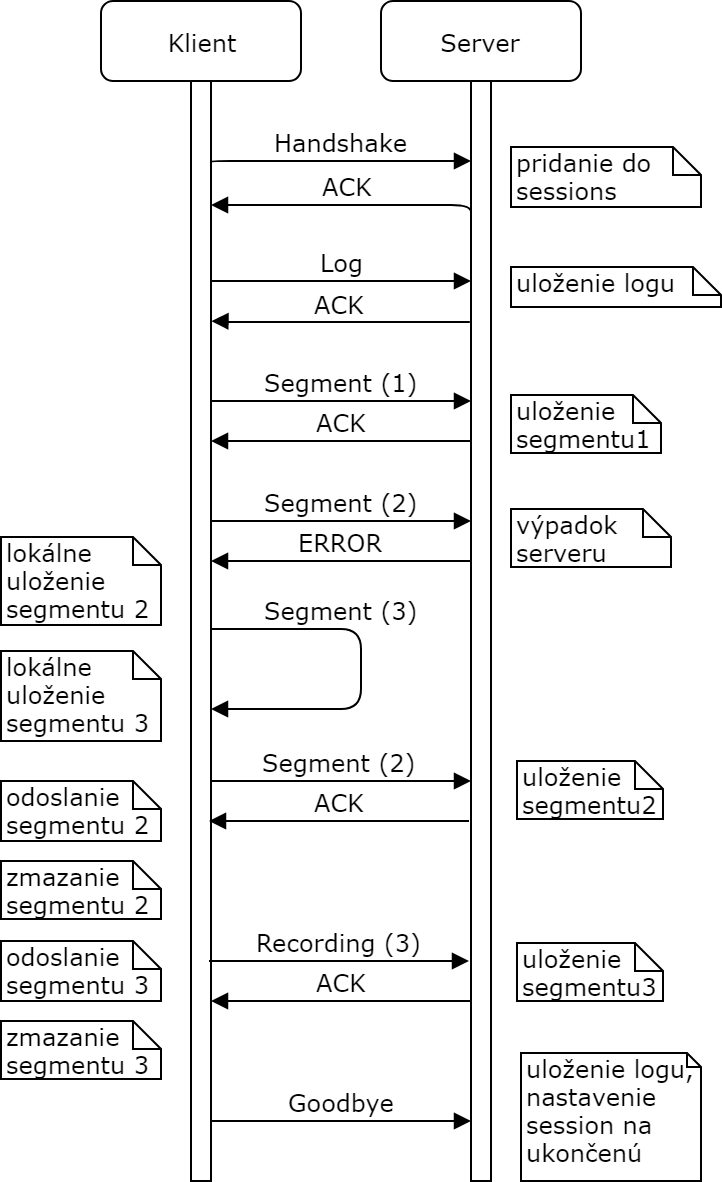
\includegraphics[width=0.6\textwidth]{obrazky-figures/protocol.png}
	\caption{Ukážka komunikácie pomocou protokolu. Komunikácia začína úvodnou požiadavkou, kde si server uloží klienta do zoznamu sessions, následne od neho prijme log a segment nahrávky. Pri prijatí ďalšieho segmentu však nastáva strata pripojenia a server klientovi už nepotvrdzuje úspešné prijatie. Klient si neodoslaný segment ukladá, avšak medzitým má už nahraný ďalší. Ak by ho ihneď odoslal, nastala by vo výslednom zázname medzera a došlo by k zámene poradia. Segment si teda ukladá a v tomto momente má už uložené dva segmenty, ktoré sa pokúsi odoslať opätovne. Po úspešnom odolaní ich z pamäte zariadenia maže. Spojenie je ukončené odoslaním klientského logu a nastavením session na ukončenú.}
	\label{protocol-example}
\end{figure}
\clearpage

\subsection{Procesy}
\label{recording-and-sending}
\FloatBarrier
\begin{figure}[!hbt]
	\centering
	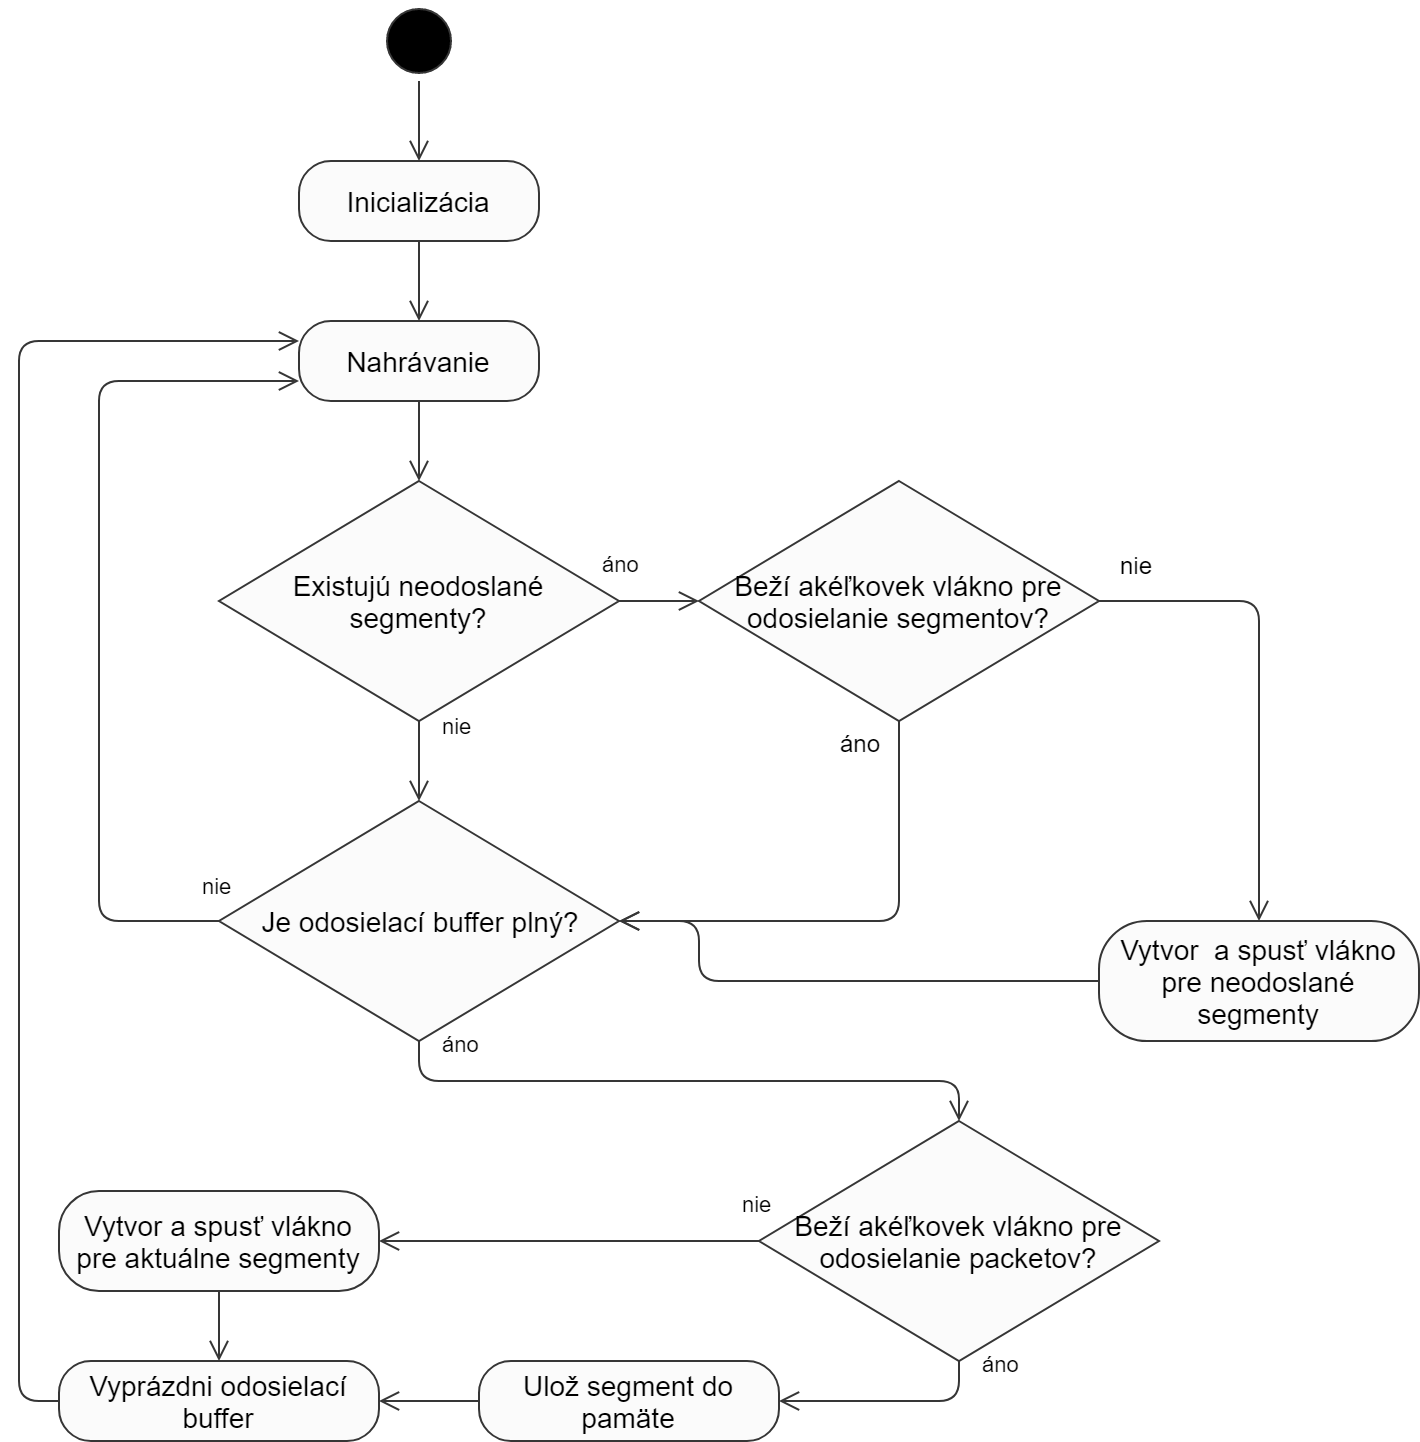
\includegraphics[width=1\textwidth]{obrazky-figures/main-recording-process.png}
	\caption{Chovanie nahrávacieho vlákna aplikácie. Spúšťa sa pri začiatku nahrávania a podľa potreby tvorí typy odosielacích vlákien, pomocou ktorých sa na server dostanú logy a segmenty. V diagrame sa vyskytujú dva typy segmentov. Aktuálne segmenty označujú časti nahrávky, ktoré sa práve dostali do odosielacieho buffru. Neodoslané segmenty vznikajú pri situácii, keď sa aktuálny segment nepodarí odoslať na server a aplikácia ho ukladá lokálne do pamäte.}
	\label{main-recording-process}
\end{figure}
\FloatBarrier

Zjednodušené fungovanie aplikácie je znázornené na obrázku~\ref{main-recording-process}. Najprv budú popísané základné stavebné prvky procesu a potom detaily postupnosti udalostí. 

Jadrom je nahrávacie vlákno, v ktorom prebieha nahrávania audia do buffru v nekonečnom cykle, ktorý sa dá prerušiť len signálom pri prerušení nahrávania alebo zvolením možnosti pre ukončenie aplikácie. V tomto cykle je potrebné zaručiť minimum akcií, ktoré trvajú čo najkratšiu dobu, pretože ak nastane nejaké čakanie spôsobené napríklad blokujúcou operáciou, preruší sa snímanie audia zo zdroja a môže dôjsť k strate vzoriek. Práve preto sa odosielanie segmentov, logov a čakanie na odpovede od servera nemôže vykonávať v nahrávacom vlákne. Podľa potreby sa v nahrávacom cykle vytvárajú pre odoslanie audia dva základné typy vlákien.

Primárne vlákno pre odosielanie aktuálnych segmentov je aj najčastejší typ vytvoreného vlákna v aplikácii. Jeho hlavným účelom je odoslanie segmentu a poprípade zabezpečenie jeho uloženia, pokiaľ odoslanie nebolo úspešné. Majú relatívne krátku životnosť a sú vytvárané vždy, keď je potrebné odoslať aktuálne nahrané audio na server. V jednom momente môže bežať len jedno vlákno pre odosielanie aktuálne nahraného segmentu. Ak by sa nahral ďalší segment ešte predtým, než sa predošlý stihol odoslať, nový segment sa uloží do lokálneho úložiska na neskoršie odoslanie.

V prípade odosielania segmentov, ktoré sú uložené v pamäti zariadenia z dôvodu zlyhania odoslania alebo prijatia serverom sa vytvára typ vlákna, ktorého inštancia beží vždy len jedna. Toto vlákno sa stará o odoslanie všetkých segmentov, ktoré sú uložené v lokálnej pamäti. Beží dlhodobo a jeho činnosť skončí vtedy, keď už nemá čo odosielať alebo sa ukončí nahrávanie, poprípade aplikácia.

Je dôležité podotknúť, že tieto dva typy vlákien nemôžu za žiadnych okolností bežať zároveň, vždy len jedno z nich. Toto obmedzenie je zavedené z dôvodu, že v momente spustenia odosielania viacerých segmentov, ktoré sú distribuované do samostatných vlákien pri kvalitnom internetovom pripojení nevznikajú problémy s poradím doručenia. Pri nestabilnom alebo pomalom pripojení však nie je možné zaistiť, aby sa doručili v rovnakom poradí, v akom boli spustené.

Ďalšia časť sekcie obsahuje detailný popis procesu na obrázku~\ref{main-recording-process}. Po overení všetkých nastavení v rámci aplikácie, spustení nahrávacieho vlákna, inicializácii objektov pre nahrávanie a odosielanie sa vytvára jednoznačný identifikátor session, ktorý je tvorený užívateľsky zvoleným názvom zariadenia a časovým údajom z počiatku nahrávania. Tento identifikátor je jedinečný pre každé nahrávanie, čiže pri zastavení nahrávania a opätovnom spustení sa generuje nový identifikátor. Vytvoria sa zložky v pamäti zariadenia, do ktorých sa môžu ukladať neodoslané segmenty a logy.

Spojenie so serverom je inicializované počiatočným odoslaním požiadavky na server, ktorá obsahuje identifikátor zariadenia (handshake). Absencia odpovede na túto požiadavku nijak neovplyvní aktivitu vlákna a pokračuje ďalej. Situácia, pri ktorej na začiatku nahrávania nie je prítomný server je bližšie popísaná v sekcii~\ref{serverless-recording}. V užívateľskom rozhraní sa zmení indikátor pripojenia na server na aktívne (len pri úspešnom handshake) a do notifikácií pribudne perzistentná notifikácia o priebehu nahrávania, ktorá nesie aj informáciu o tom, či je momentálne nadviazané spojenie so serverom. Notifikácia je aktívna počas celej doby nahrávania a prezentuje sa aj vo forme ikonky v hornej lište zariadenia. Bez ohľadu na to, či sa handshake podaril alebo nie, sa po inicializácii buffru a začatí nahrávania vstupuje do nahrávacieho cyklu.

V cykle sa periodicky napĺňa odosielací buffer hodnotami nahraných vzoriek. Prioritne sa kontroluje obsah zložky s neodoslanými segmentami, avšak to len v prípade, že prebehol handshake (bez handshake server nemá zaregistrovanú aktuálnu session a nevedel by kam ukladať neodoslané segmenty), zariadenie je online a nebeží nijaké vlákno pre odosielanie aktuálnych alebo neodoslaných segmentov (pre zachovanie správneho poradia odosielania). Pokiaľ sú tieto podmienky splnené, je potrebné neodoslané segmenty ihneď odoslať a počas ich odosielania neustále nahrávať nové segmenty, ktoré sa ale budú ukladať do pamäte zariadenia. Odoslanie týchto neodoslaných segmentov v správnom poradí a čo najrýchlejšie zabezpečuje inštancia vlákna pre neodoslané segmenty. Tento proces je detailnejšie vysvetlený v sekcii~\ref{sending-unsent} o odosielaní segmentov z pamäti. Pokiaľ neexistujú žiadne neodoslané segmenty, skontroluje sa, či nehrozí pretečenie odosielacieho buffru. Pokiaľ áno, musí sa jeho obsah (segment) odoslať na server a vyprázdniť predtým, než sa do neho začnú zapisovať nové vzorky. 

Pred odoslaním segmentu sa kontroluje internetové pripojenie, zároveň sa aj kontroluje, či prebehol handshake. Ak neprebehol, spustí sa vlákno pre handshake. Než nastane samotné vytvorenie a spustenie vlákna pre odoslanie aktuálneho segmentu, musia byť splnené isté požiadavky. Pri porušení aspoň jeden z nich sa namiesto odoslania segment ukladá do lokálnej pamäte. Medzi tieto požiadavky patrí neprítomnosť akýchkoľvek neodoslaných segmentov, úspešný handhshake a nesmie bežať nijaké odosielacie vlákno. Ak ani jedna podmienka nie je porušená, tak sa vytvorí nové vlákno, ktorého jedinou zodpovednosťou je odoslanie daného aktuálneho segmentu. Ten sa pokúsi uskutočniť odoslanie a pri neúspechu segment ukladá do lokálnej pamäte zariadenia, odkiaľ sa neskôr bude môcť odoslať opäť. Pri úspešnom odoslaní vlákno zaniká.


\subsection{Offline funkcionalita}
\label{serverless-recording}

Aplikácia obsahuje možnosť nahrávania a vytvorenie úplnej nahrávky z jej segmentov aj bez prítomnosti servera. Táto funkcia je vhodná napríklad pre krátke nahrávanie, kde server nemusí byť k dispozícii a zároveň sprostredkúva plnohodnotný offline chod aplikácie. Nastáva pri započatí nahrávania, kde sa nepodarí získať odpoveď servera na handshake.

Pri tejto situácii sa nastaví premenná, ktorá udržuje informáciu o tom, či handshake prebehol. Nahrávanie potom pokračuje podobným spôsobom, ako pri úspešnom handshake, avšak so zopár rozdielmi. V nahrávacom cykle sa budú naviac periodicky odosielať požiadavky o handshake. Handshake požiadavky sa odosielajú vždy pred akciou, ktorá zahŕňa komunikáciu so serverom. V nahrávacom cykle sa teda handshake odosiela v momente, keď sa naplní odosielací buffer (vzniká segment) a pri prítomnosti spojenia so serverom (handshake), by sa odoslal na server. Kontrola na neodoslané segmenty je vynechaná, rovnako ako aj pokus odoslania obsahu odosielacieho buffru na server. Namiesto toho sa obsah odosielacieho buffru (segment) rovno ukladá do úložiska zariadenia.

Ak sa v priebehu nahrávania podarí pripojiť na server a prebehne úspešný handshake, všetky segmenty sú prioritne v správnom poradí odoslané na server, kým nové sa nahrávajú a nenastane žiadna medzera. Je použité vlákno pre neodoslané segmenty. Po odoslaní všetkých nahrávok nahrávanie pokračuje štandardným spôsobom.

V prípade, že sa nahrávanie ukončí a handshake stále neprebehol, v pamäti zariadenia sa budú nachádzať segmenty nahrávky, ktorých množstvo závisí na veľkosti odosielacieho buffru. Tieto však výslednú nahrávku tvoria až po ich poskladaní, čo je funkcia servera. Aplikácia umožňuje danú nahrávku poskladať aj lokálne, bez prítomnosti servera. Táto možnosť sa označuje ako kompozícia nahrávky a nachádza sa v menu aplikácie.

Po zvolení tejto možnosti sa otvorí prehliadač zložiek, kde je očakávaná voľba zložky s nahrávkami. Táto zložka musí byť vytvorená v rámci nahrávania a nemôže byť prázdna. V zložke sa z jednotlivých súborov (segmentov), vytvorí konečná nahrávka, ktorá je umiestnená do špeciálnej zložky. Po úspešnej kompozícii sa na obrazovku vypíše informácia o stave a umiestnení tejto nahrávky. Pri opätovnej kompozícii sa výsledok predošlej kompozície s rovnakým názvom prepíše. Kompozícia nijakým spôsobom nemodifikuje ani nemaže segmenty, vytvára iba konečnú nahrávku, ktorá je oddelená od jej segmentov. Pri opätovnom chode aplikácie a úspešnom odoslaní jednotlivých neodoslaných segmentov sa segmenty mažú, avšak zložka s výslednou nahrávkou ostáva nedotknutá.


\subsection{Opätovné odosielanie}
\label{sending-unsent}

\begin{figure}[!hbt]
	\centering
	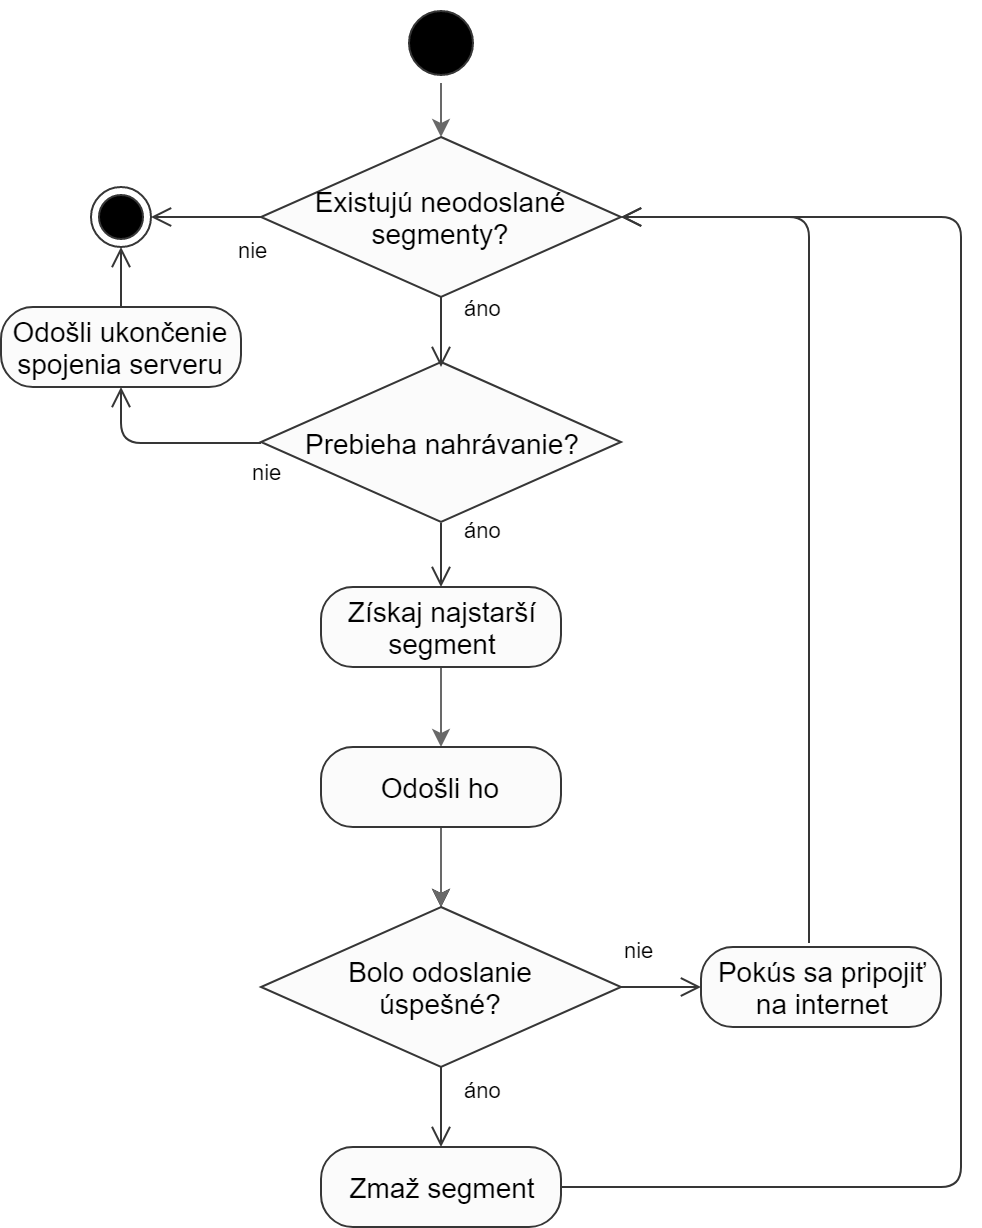
\includegraphics[width=0.6\textwidth]{obrazky-figures/sending_unsent.png}
	\caption{Odosielanie záznamov uložených v pamäti v rámci aktuálneho nahrávania.}
	\label{sending-unsent-pic}
\end{figure}


Segmenty, ktoré sa neodoslali na server na prvý pokus sú uložené v lokálnom úložisku. Rozlišujú sa dva základné typy neodoslaných segmentov. Prvý predstavuje neodoslané segmenty v rámci aktuálne bežiaceho nahrávania, ktoré môžu vzniknúť výpadkom internetového pripojenia alebo servera. Pri opätovnom ustanovení spojenia sa tieto segmenty prioritne odosielajú na server. Druhý typ predstavuje neodoslané segmenty, ktoré sú súčasťou už ukončeného nahrávania. Vznikajú pri prebehnutí nahrávania bez prítomnosti servera alebo z dôvodu ukončenia nahrávania predtým, než sa stihli odoslať všetky segmenty z lokálneho úložiska.

V prípade neodoslaných segmentov v rámci \textbf{aktuálne bežiaceho nahrávania} je chovanie odosielacieho vlákna pre neodoslané segmenty znázornené na obrázku~\ref{sending-unsent-pic}.
Odosielacie vlákno odosiela záznamy uložené v pamäti, kým tam už nijaké nie sú a potom ukončí svoju činnosť. Jeho činnosť sa preruší aj pri ukončení aplikácie alebo nahrávania. Po jeho spustení sa hneď dostáva do cyklu, v ktorom kontroluje prítomnosť neodoslaných segmentov. Súbory s neodoslanými segmentmi sú pomenované číselne, hodnota sa vždy inkrementuje. 

Najstarší segment získa pomocou súboru, ktorého názov je čo najmenším číslom. Pri neúspešnom odoslaní prebieha pokus o pripojenie k internetu (zapnutie Wi-Fi pri detekcii vypnutia). Pri úspešnom odoslaní sa segment zmaže. V oboch prípadoch cyklus potom pokračuje od začiatku, kým sa neodošlú všetky súbory a pokiaľ beží nahrávanie.

Toto vlákno pracuje v cykle kvôli tomu, že pri výpadku pripojenia nie je možné s istotou určiť, za akú dobu bude aplikácia mať opäť pripojenie k internetu a v momente pripojenia začne odosielanie segmentov z úložiska okamžite. 


\label{previous-recording}
Druhým typom neodoslaných segmentov sú \textbf{segmenty z predošlých nahrávaní}, ktoré sa už v minulosti ukončili predtým, než sa všetky ich segmenty dostali na server. Pokus o ich spätné odoslanie prebieha pri každom štarte aplikácie alebo zmene ukladacej zložky, kedy je vykonaná kontrola nad zložkou. Pokiaľ už v zložke súbory z predošlých sessions sú, skontroluje sa každá na prítomnosť neodoslaných segmentov. Tie sa potom spätne odosielajú na server.

Server danú session môže mať zaregistrovanú, alebo ju vôbec nemusí poznať, čo sa môže stať, pokiaľ nedôjde k handshake alebo je session manuálne odstránená zo servera. Tieto segmenty sa na server odosielajú so špeciálnym označením, aby server vedel, že nemá nastaviť dané spojenie na aktívne, ale iba dostáva dodatočné segmenty z už ukončeného nahrávania. Odosielajú sa aj logy, ktoré sú taktiež označené. Všetky segmenty pridáva na koniec už existujúcej nahrávky, pretože sa nemôže stať situácia, kedy by sa doručovali segmenty z nahrávania, aj keď v úložisku sú stále neodoslané segmenty. Vždy sa prioritne odosiela obsah úložiska, čiže toto spätné odosielanie nezapríčiní narušenie poradia segmentov v nahrávke. Ukončenie spätného odosielania je podobné ukončeniu normálneho nahrávania. Segmenty sú vždy po úspešnom odoslaní zmazané z úložiska.


Pokiaľ server session nepozná, vytvorí si záznam do zoznamu sessions, ktorý označí ako ukončený a prijíma jednotlivé segmenty. Vytvorí sa aj zložka pre danú session. Po ukončení odosielania do logu zapíše informáciu o úspechu. Od klienta sa mu dostane jeho verzia logu ako pri klasickom ukončení nahrávania. 


Dôležitou záležitosťou je aj zabezpečenie, aby takéto spätné odosielanie nijak nenarušilo chod aplikácie a nezasahovalo do chodu nahrávania alebo ukladania v rámci potenciálne bežiacej session. Oddelenie spätného a aktuálneho odosielania je zabezpečená pomocou samostatného vlákna, ktoré sa stará o spätné odosielanie a nikdy neodosiela záznamy z aktuálne prebiehajúceho nahrávania. Pri prechádzaní jednotlivých zložiek pre sessions sa vždy skontroluje prítomnosť aktuálneho nahrávania. Pokiaľ nahrávanie prebieha a narazí sa na zložku tohto nahrávania, je vynechaná a nespracúva sa. Spätné odosielanie segmentov predošlých sessions je teda úplne izolované od aktuálneho nahrávania a všetkých akcií, ktoré v ňom prebiehajú.

Týmto procesom sa zaisťuje, že po výpadku alebo chodu aplikácie bez prítomnosti servera sa nahrané záznamy stále dokážu synchronizovať so serverom a nič neostane iba v úložisku zariadenia. Špeciálny prípad nastáva, ak nahrávanie prebehne do špecifickej zložky a užívateľ ju už nikdy v budúcnosti nezvolí ako úložisko. V tomto prípade sa už segmenty neodošlú, keďže rekurzívne prehľadávať každú zložku v celom úložisku na zariadení by bolo príliš náročné na zdroje.

\subsection{Ošetrenie výpadkov pripojenia}

Pri behu aplikácie sa môže stať, že sa stratí internetové pripojenie, či už vypnutím Wi-Fi, stratou signálu alebo výpadkami. Aj s týmto aplikácia počíta a dané stavy rieši. Pri vypnutí Wi-Fi je okamžite opätovne spustené, aj pri periodickom vypínaní. Ak je zariadenie pripojené na Wi-Fi, avšak nemá prístup k internetu, nespôsobí to nijaké problémy a aplikácia po obnovení pripojenia beží očakávaným spôsobom (odošle všetky nahrané segmenty). Pri odosielaní jednotlivých požiadaviek na server je obmedzený čakací limit. Pokiaľ sa nedarí dostať odpoveď od servera, nastáva blokovanie po maximálnu dobu čakacieho limitu, to však prebieha vždy v samostatnom vlákne, takže nijak neovplyvňuje nahrávanie a funkcionalita je zachovaná aj pri pomalom alebo nestabilnom internetovom pripojení. Žiadne obmedzenia týkajúce sa doby behu aplikácie bez pripojenia neboli implementované.

\subsection{Logovanie}

Počas celého behu aplikácie sa aktívne zaznamenávajú všetky dôležité udalosti alebo chybové stavy. Loguje sa na serveri a aj na zariadení, pričom každá session má vlastný súbor s logom. Pri ideálnom chode aplikácie, sa obsahy logov na serveri a na mobilnom zariadení zhodujú.

Nečakané alebo chybné stavy môžu byť dôvodom rozdielov v logoch. Napríklad pri výpadku pripojenia sa loguje iba na klientskej časti a týmto spôsobom vznikajú odlišnosti. Logy dodržujú presný formát, ktorý sa skladá z informácie o čase, názvu session, počtu sekúnd od počiatku nahrávania a správy. Logy sa delia na také, ktoré môžu vzniknúť iba na klientovi a na spoločné.
Medzi spoločné logy patria napríklad informácie o:
\begin{itemize}
  \item{vytvorení buffru,}
  \item{inicializácie objektu pre nahrávanie (zahrnutá je aj konfigurácia nastavení pri nahrávaní a aktuálna verzia aplikácie),}
  \item{spustení nahrávania,}
  \item{ukladaní záznamov do pamäte zariadenia,}
  \item{úspešnom opätovnom odoslaní segmentov,}
  \item{chybách pri otváraní súborov so segmentmi,}
  \item{úspešnom ukončení nahrávania,}
  \item{spätnom odosielaní segmentov z predošlých sessions,}
  \item{správnom uložení neodoslaného segmentu.}
\end{itemize}
Logy, ktoré sú špecifické iba pre logovací súbor klienta nesú informácie o:
\begin{itemize}
  \item{neúspešnom handshake,}
  \item{neodoslaní segmentu,}
  \item{poruchách pripojenia,}
  \item{chybách pri vytváraní súborov alebo zložiek,}
  \item{neúspech pri spätnom odosielaní,}
  \item{pokusoch o zapnutie Wi-Fi.}
\end{itemize}

Zoznam logovaných položiek vznikal prirodzene pri vyvíjaní aplikácie, pretože logovací súbor bol použitý ako jeden z nástrojov pre riešenie chybových stavov alebo nečakaných reakcií aplikácie.


\chapter{Nahrávanie audia}
\label{nahravanie}

V tejto kapitole budú vysvetlené metódy prevodu analógového zvuku na digitálny, formát uloženia audia v digitálnej podobe, atribúty ovplyvňujúce kvalitu a veľkosť zvukového záznamu. Poskytuje fundamentálne znalosti, ktoré sú potrebné pre hlbšie pochopenie manipulácie a nahrávania audia, či už na Androide alebo na iných operačných systémoch.


\section{A/D prevodník}
\label{ad_prevodnik}

Pre prevod analógového (spojitého) zvuku na digitálny (diskrétny) slúži elektronická súčiastka, ktorá sa nazýva A/D prevodník. Spracovanie alebo ukladanie audia je možné len v jeho digitálnej podobe. Zvuk sa šíri vlnením istej hmoty (napríklad vzduch) a vznikom vibrácií. Prevodník zaznamenáva neustále sa meniace napätie spôsobené zvukovými vibráciami a vo vopred stanovených intervaloch meria napätie mikrofónu. Po meraní priradí magnitúde napätia číselnú hodnotu \cite{Lathi}. Keďže konverzia zahŕňa diskretizáciu oboru hodnôt signálu, nevyhnutne zavádza malé množstvo chyby a šumu. Opačnú konverziu (z digitálneho zvuku na analógový) sprostredkúva D/A prevodník.



\section{Pulzná kódová modulácia}
\label{PCM}

Pulzná kódová modulácia (ďalej už len PCM) je metóda prevodu analógového signálu na digitálny. Využíva A/D prevodník na pravidelné prečítanie hodnoty signálu, ktorú potom ukladá v binárnej podobe. Vernosť digitálneho záznamu k analógovému určujú dve základné premenné: vzorkovacia frekvencia a bitová hĺbka. 

\subsection*{Vzorkovacia frekvencia}

Definuje počet prečítaných vzoriek analógového signálu za určitú jednotku času (zvyčajne sekunda) pri jeho premene na digitálny signál. Jednotka vzorkovacej frekvencie je 1 hertz~(Hz) a ľudské ucho je typicky schopné zachytiť frekvencie od 20 do 20 000 Hz  \cite{Physics4}.

Ako je zrejmé z obrázku~\ref{sampling-comparison}, vyššia vzorkovacia frekvencia znamená:
\begin{itemize}
  \item{zber väčšieho množstva informácií,}
  \item{presnejší obraz pôvodného signálu,}
  \item{lepšia kvalita zvuku,}
  \item{väčší objem súborov,}
  \item{dlhšie a náročnejšie spracovanie.}
\end{itemize}

\begin{figure}[hbt]
	\centering
	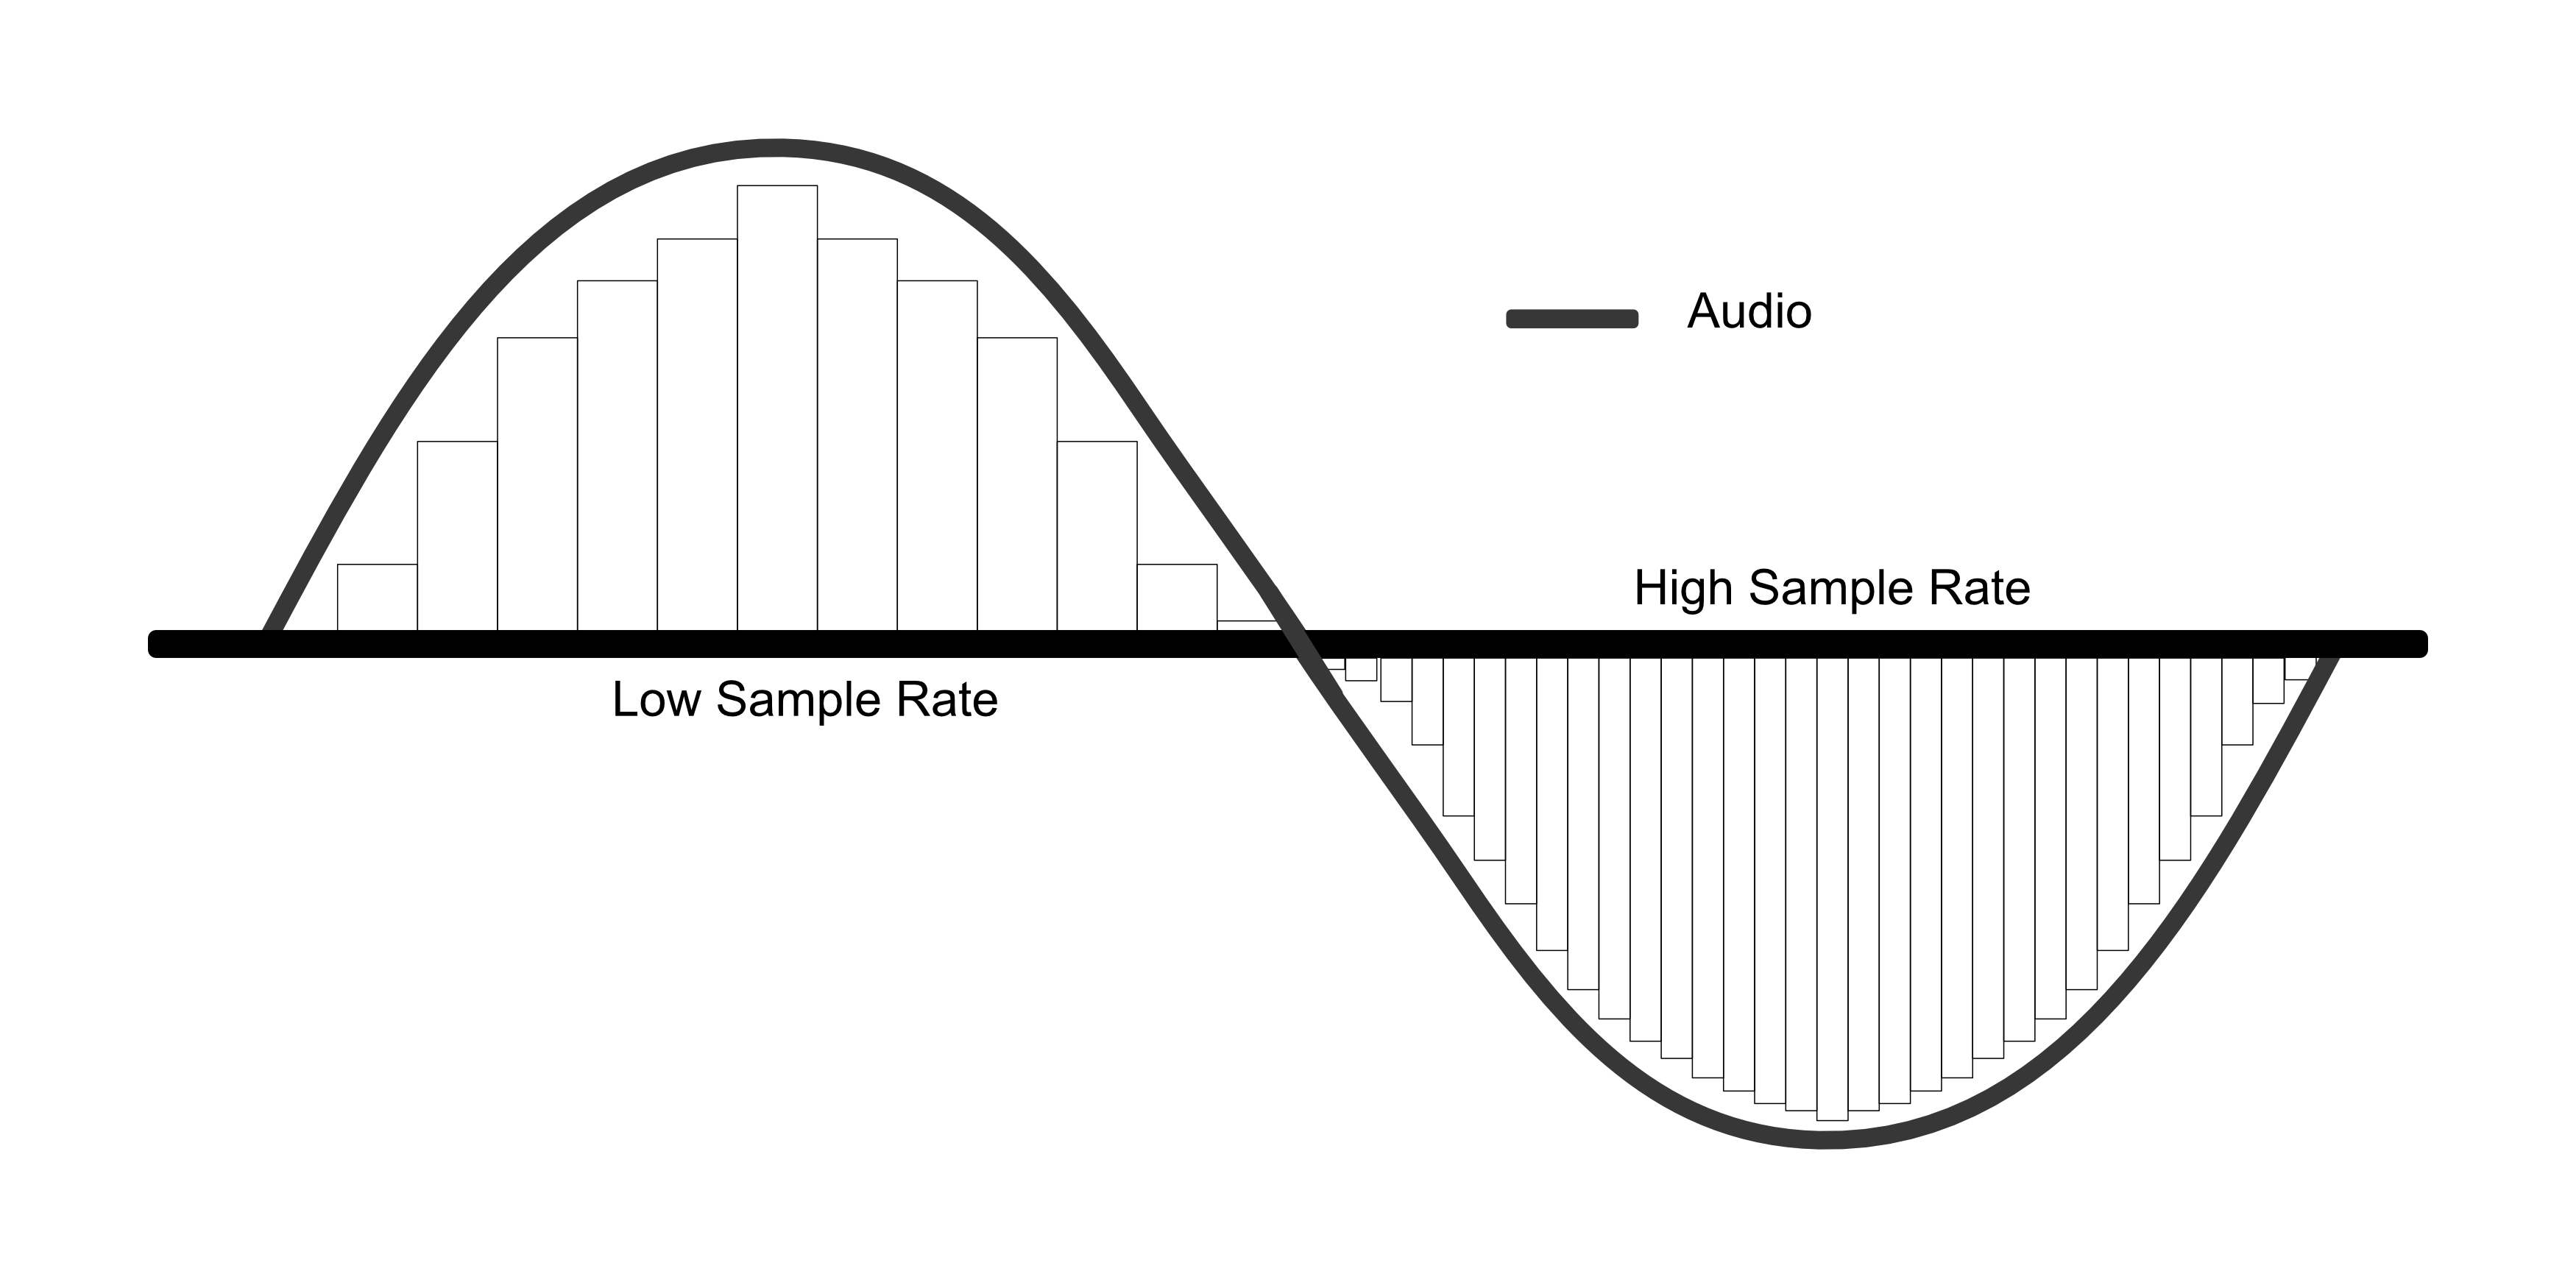
\includegraphics[width=0.8\textwidth]{obrazky-figures/sampling-comparison.png}
	\caption[Porovnanie kvality audia pri rôznych hodnotách vzorkovacej frekvencie.]%
    {Porovnanie hodnôt vzorkovacích frekvencií\protect\footnotemark.}
	\label{sampling-comparison}
\end{figure}



\footnotetext{https://www.masteringthemix.com/blogs/learn/113159685-sample-rates-and-bit-depth-in-a-nutshell}


V praxi sa najčastejšie stretávame s frekvenciami 44.1~kHz, 48~kHz, 88.2~kHz, 96~kHz, 192~kHz. 


\subsection*{Bitová hĺbka}
Počet bitov v každej zaznamenanej vzorke. Označuje teda kvalitu alebo rozlíšenie vzorky. Napríklad, zvuk na kompaktnom disku požíva bitovú hĺbku 16, pričom DVD alebo Blu-ray využíva 24 bitovú hĺbku. Zmeny v bitovej hĺbke ovplyvňujú primárne pomer signálu k šumu a dynamický rozsah, avšak techniky ako dithering (algoritmus prevodu na nižšiu kvalitu s potlačením nežiadúcich javov), oversampling (vzorkovanie na frekvencii oveľa vyššej než je potrebná pre rekonštrukciu) alebo tvarovanie šumu (technika zvyšovania pomeru signálu k šumu) zmierňujú tieto negatívne účinky aj bez zmeny hĺbky bitov. Bitová hĺbka ovplyvňuje aj veľkosť súboru a tým pádom rýchlosť prenosu dát. Zmysel dáva len pri PCM digitálnom signále, pretože iné, často stratové formáty nemajú asociované bitové hĺbky. 
	


\chapter{Vývoj na Androide}
\label{development_android}

\section{Nahrávanie v Androide}
\label{recording_android}

Android SDK (súbor nástrojov pre vývoj na Androide) poskytuje mnoho možností ako využívať funkcie mobilných zariadení. Výnimkou nie je ani nahrávanie audia. Na tento účel Android ponúka použitie dvoch rozhraní, ktoré fungujú veľmi podobne, avšak v spracovaní výsledného audia ponúkajú odlišné prístupy. 

\subsubsection{MediaRecorder}

\texttt{MediaRecorder} je najrozšírenejším spôsobom ako nahrávať na Androide nielen audio, ale aj video. Proces inicializácie a nahrávania je znázornený pomocou stavového diagramu na obrázku~\ref{mediarecorder-states}. \texttt{MediaRecorder} pred spustením nahrávania audia vyžaduje špecifikáciu zdroja audia, formátu výstupného audia, audio kódeku a súbor pre výstup.

Pre účel tejto práce je teda menej vhodné použitie triedy \texttt{MediaRecorder}, keďže medzi jeho vlastnosti patrí ukladanie nahraného audia do súboru \cite{Mednieks}, čo je nežiadúce, keďže jedným z cieľov práce je predísť obmedzeniu nízkych kapacít mobilných zariadení a čo najviac sa vyhnúť ukladaniu priamo na zariadenie. Z toho dôvodu je popísaný len okrajovo. 

\begin{figure}[hbt]
	\centering
	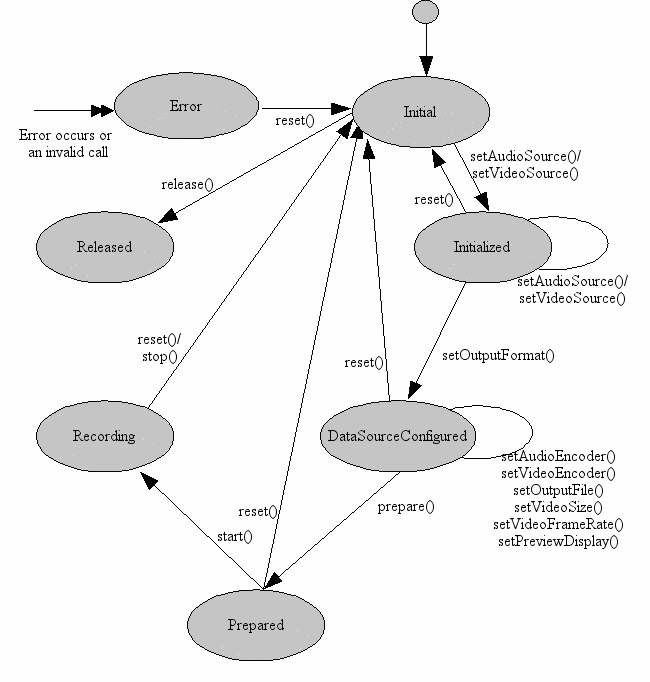
\includegraphics[width=0.8\textwidth]{obrazky-figures/mediarecorder.png}
	\caption{Stavový diagram pre \texttt{MediaRecorder}\protect\footnotemark.}
	\label{mediarecorder-states}
\end{figure}

\subsubsection{AudioRecord}

Druhým spôsob pre nahrávanie audia predstavuje \texttt{AudioRecord}. Zatiaľ bolo predstavené rozhranie pre nahrávanie s okamžitým uložením zaznamenaného audia, ale v prípade potreby spracovania dát počas nahrávania ho nie je vhodné použiť. Pre tieto účely je tu trieda \texttt{AudioRecord}. Pri jej použití Android neukladá audio dáta do súboru, avšak využíva interný buffer \cite{Komatineni}. To umožňuje programátorovi s dátami manipulovať a spracovávať ich. 

Inicializácia \texttt{AudioRecord} objektu vyžaduje informáciu o:
\begin{itemize}
  \item{zdroji audia,}
  \item{vzorkovacej frekvencii,}
  \item{zvukovom kanáli,}
  \item{audio formáte,}
  \item{veľkosti buffru.}
\end{itemize}

\subsubsection{Zdroj audia}

\footnotetext{https://developer.android.com/reference/android/media/MediaRecorder}

\texttt{AudioRecord} podporuje množstvo zdrojov audia, z ktorých vie nahrávať, medzi najpoužívanejšie nastavenia zdroja audia patria:

\begin{itemize}
  \item{\texttt{MIC} (mikrofón),}
  \item{\texttt{CAMCORDER} (zdroj zvuku ladený na nahrávanie videa, s rovnakou orientáciou ako fotoaparát),}
  \item{\texttt{REMOTE\_SUBMIX} (používaný na zaznamenávanie mixov audio tokov, ktoré sú vysielané do vzdialeného prijímača),}
  \item{\texttt{VOICE\_CALL} (nahrávanie volaní),}
  \item{\texttt{VOICE\_RECOGNITION} (zdroj zvuku ladený na rozpoznávanie reči).}
\end{itemize}

V rámci aplikácie je vždy použitá možnosť \texttt{MIC}, ktorá podporuje aj externé nahrávanie po pripojení k bezdrôtovému zdroju. Nastavenie \texttt{VOICE\_RECOGNITION} sa môže zdať ako vhodná možnosť, avšak pri tomto nastavení audio prechádza spracovaním a niektoré úrovne zvuku môžu byť vyhodnotené ako nepotrebné pre rozoznanie reči a vyhodené predtým, než by sa dostali cez rozhranie do aplikácie.

\subsubsection{Vzorkovacia frekvencia}

Požaduje sa udanie v hertzoch a udáva počet zvukových vzoriek na každý kanál za sekundu. Frekvencia 44 100~Hz má garanciu fungovania na všetkých zariadeniach. Ostatné frekvencie môžu, ale nemusia byť podporované a zisťuje sa to pomocou funkcie, ktorá pre konkrétnu vzorkovaciu frekvenciu, audio formát a konfiguráciu zvukového kanálu vráti negatívnu hodnotu, ak je nahrávanie v tejto kombinácii nepodporované na zariadení. 

\subsubsection{Zvukový kanál}

Existuje veľa nastavení zvukového kanálu, avšak tieto majú garanciu fungovania na každom zariadení:

\begin{itemize}
  \item{\texttt{CHANNEL\_IN\_MONO} (jeden zvukový kanál),}
  \item{\texttt{CHANNEL\_IN\_STEREO} (viac zvukových kanálov, typicky dva).}
\end{itemize}

\subsubsection{Audio formát}

Popisuje bitovú reprezentáciu nahraných dát, teda bitovú hĺbku. Podporované sú:

\begin{itemize}
  \item{\texttt{ENCODING\_PCM\_8BIT} (každá vzorka predstavuje 8 bitové kladné celé číslo v rozsahu [0, 255] s 128 posunom pre 0),}
  \item{\texttt{ENCODING\_PCM\_16BIT} (každá vzorka predstavuje 16 bitové celé číslo v rozsahu [-32 768, 32 767]),}
  \item{\texttt{ENCODING\_PCM\_FLOAT} (uvedené až v neskoršej verzii Androidu, reprezentuje 32 bitové vzorky).}
\end{itemize}

\subsubsection{Veľkosť buffru}

Označuje veľkosť (v bajtoch) interného buffru, do ktorého sa bude nahrávať. \texttt{AudioRecord} trieda poskytuje internú metódu, ktorá na základe konfigurácie dokáže určiť minimálnu veľkosť interného buffru. Táto hodnota je minimum potrebné pre ukladanie vzoriek s určitou frekvenciou, počtom kanálov a bitovou hĺbkou, takže zníženie veľkosti buffra pod túto hranicu vedie k zlyhaniu inicializácie objektu \texttt{AudioRecord}.

\section{Štruktúra projektu}
\label{android_structure}

Pre lepšie pochopenie jednotlivých častí projektu je dobré poznať štruktúru typickej Android aplikácie vyvíjanú v prostredí Android Studio. Zobrazenie štruktúry priamo v Android Studio neodzrkadľuje nutne skutočné usporiadanie súborov projektu, ale je usporiadané podľa modulov a typov súborov. Uľahčuje sa tým navigácia medzi kľúčovými súbormi v projekte. Medzi zmeny v štruktúre patrí napríklad:
\begin{itemize}
\item{všetky konfiguračné súbory sú zoskupené v zložke Gradle Scripts, ktorá je na najvyššej úrovni,}
\item{manifesty zoskupené na najvyššej úrovni (uľahčenie orientácie, ak existuje viacero modulov s viacero manifestami),}
\item{alternatívne zdrojové súbory sú zoskupené podľa typu.}
\end{itemize}



\begin{figure}[!hbt]
	\centering
	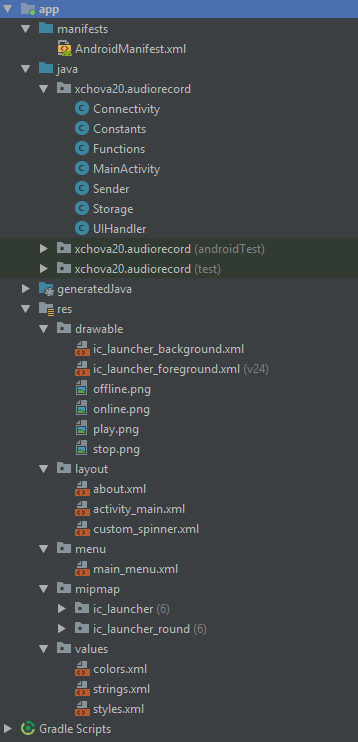
\includegraphics[width=0.5\textwidth]{obrazky-figures/structure-example.png}
	\caption{Štruktúra Android aplikácie. Všetky moduly sú uložené v zložke Java. XML súbory predstavujú vizuálnu štylizáciu prvkov v užívateľskom rozhraní, vzhľad menu a definície štýlov, farebnej schémy alebo textových reťazcov v rámci XML súborov.}
	\label{structure-example}
\end{figure}

V nasledujúcej časti bude vysvetlená podstata jednotlivých častí projektu, ako sú viditeľné na obrázku~\ref{structure-example}.

\subsection*{Manifest}
\label{manifest}

Každý projekt musí obsahovať manifest súbor. Manifest obsahuje informácie o projekte, ktoré využívajú nástroje zostavovanie projektu, operačný systém Android a aj Google Play (obchod s aplikáciami). Manifest je povinný uviesť následovné:
\begin{itemize}
\item{názov balíka, v ktorom sa nachádza aplikácia,}
\item{komponenty aplikácie (aktivity, služby, poskytovateľov obsahu),}
\item{oprávnenia, ktoré aplikácia potrebuje,}
\item{požiadavky na hardvér a softvér.}
\end{itemize}

\subsection*{Java}

Najdôležitejšia zložka, ktorá obsahuje všetky zdrojové kódy oddelené podľa názvov príslušných balíkov a sú tu zahrnuté aj testy. Testy sú rozdelené na jednotkové (unit testy) a inštrumentačné (instrumented testy). Jednotkové testy izolujú jednotlivé testované komponenty od ich závislostí, inštrumentačné testy sprostredkúvajú integračné testovanie aplikácie s možnosťou kontrolovania životného cyklu aplikácie. 

\subsection*{Res}

Všetky zdroje, ktoré nemajú charakter kódu sa ukladajú do tejto zložky. Najčastejšie ide o: 
\begin{itemize}
\item{bitmapové súbory (.png, .jpg, .gif)\protect\footnotemark alebo XML súbory, ktoré sa dajú kompilovať do rôznych grafických formátov (zložka drawable),}
\item{definícia vzhľadov komponentov užívateľského rozhrania (zložka layout),}
\item{ikony (zložka mipmap),}
\item{XML súbory, ktoré obsahujú jednoduché hodnoty (reťazce, čísla, farby), primárne slúžiace na definíciu rôznych farebných schém (konštantné hodnoty farieb používané naprieč celou aplikáciou za účelom jednotnosti), štýlov (XML definície, ktoré sa aplikujú na elementy užívateľského rozhrania), hodnôt reťazcov (hodnoty textových reťazcov použitých v aplikácii, napríklad nadpisy, popisy tlačidiel alebo možnosti v menu) a mnoho ďalších voliteľných druhov konštánt (zložka values) \cite{Jackson}.}
\end{itemize}
\footnotetext{https://developer.android.com/guide/topics/resources/providing-resources}

\section{Oprávnenia}
\label{permissions}

Oprávnenia sú nástrojom ochrany súkromia užívateľa a aplikácie musia požiadať o povolenie na prístup k určitým zdrojom, ktoré vyžadujú na chod alebo istú funkcionalitu, ktorú sprostredkúvajú v rámci ich chodu. Niektoré oprávnenia sú nevyhnutné pre beh aplikácie a po ich neudelení sa aplikácia zavrie, niektoré nie sú nutné a ich nepovolenie spôsobí stratu istej funkcionality, avšak aplikáciu je stále možné využívať. Niektoré oprávnenia sa môžu prideliť automaticky systémom, iné vyžadujú schválenie užívateľa. Medzi oprávnenia, ktoré sú pridelené automaticky patria všetky tie, ktoré nepredstavujú nijaké riziko ohrozenia súkromia, napríklad povolenie o prístup k internetovému pripojeniu alebo prístup k stavu Bluetooth. Medzi rizikové oprávnenia patrí napríklad povolenie odosielať SMS správy alebo prístup k čítaniu a zapisovaniu do úložiska. Základnou myšlienkou povolení je znemožnenie aplikáciám negatívne zasahovať do chodov iných aplikácií alebo operačného systému. Každá aplikácia je povinná deklarovať zoznam svojich požadovaných oprávnení do manifestu. 

Proces udeľovania oprávnenia sa líši na základe verzie Androidu. Ak je verzia Androidu aspoň 6.0, užívateľ v čase inštalácie aplikácie nie je informovaný o nijakých oprávneniach a ich povolenie je vyžiadané až počas behu aplikácie formou dialógového okna, v ktorom sa nachádza informácia o type oprávnenia a možnosť prijať alebo zamietnuť oprávnenie. V prípade zamietnutia oprávnenia sa pri opätovnom požadovaní daného oprávnenia zobrazí aj možnosť vypnutia akéhokoľvek budúceho žiadania tohto povolenia pre aplikáciu. 

Pri verziách Androidu nižších ako 6.0 sa proces prideľovania líši. Oprávnenia nie sú žiadané za behu aplikácie postupne, ale sú uvedené pri inštalácii a udelené naraz. To znamená, že užívateľ nemôže selektívne udeliť iba konkrétne oprávnenia tak, ako to je možné u vyšších verziách, ale môže udeliť len všetky alebo zrušiť inštaláciu aplikácie. Ak aplikácia vyžaduje dôsledkom aktualizácie nové oprávnenia, užívateľ je vyzvaný k povoleniu pred inštaláciou aktualizácie. 

Aplikácia, ktorá je predmetom tejto práce vyžaduje pre svoj chod skupinu nastavení. V nasledujúcej časti bude každé oprávnenie popísané a odôvodnené v rámci funkcionality aplikácie.

Oprávnenia, ktoré sú pridelené automaticky systémom zahŕňajú:
\begin{itemize}
  \item{\texttt{INTERNET} -- povoľuje aplikácii prístup k internetovému pripojeniu, je potrebné pre komunikáciu so serverom a odosielanie nahrávok,}
  \item{\texttt{ACCESS\_WIFI\_STATE} -- prístup k stavu Wi-Fi pripojenia, pri neúspešnom odoslaní požiadavky sa kontroluje na stav siete,}
  \item{\texttt{ACCESS\_NETWORK\_STATE} -- prístup k stavu sietí, pokiaľ je zariadenie pripojené inak ako cez Wi-Fi,}
  \item{\texttt{CHANGE\_WIFI\_STATE} -- manipulácia so stavom Wi-Fi pripojenia, využívané pre opätovné zapnutie pri detekcii vypnutia pripojenia,}
  \item{\texttt{MODIFY\_AUDIO\_SETTINGS} -- modifikácia nastavenia audia, používaná napríklad pre prepínanie mikrofónu používaného na nahrávanie,}
  \item{\texttt{BLUETOOTH} -- pripájanie sa na zariadenia cez Bluetooth, umožňuje nahrávanie cez externý mikrofón.}
\end{itemize}

Oprávnenia, ktoré vyžadujú potvrdenie od užívateľa predstavujú:
\begin{itemize}
  \item{\texttt{RECORD\_AUDIO} -- povolenie pre nahrávanie audia, toto oprávnenie je dôležité pre chod aplikácie,}
  \item{\texttt{WRITE\_EXTERNAL\_STORAGE} -- zápis a čítanie do úložiska zariadenia, taktiež dôležité oprávnenie, bez ktorého sa nemôžu ukladať logy, ani segmenty.}
\end{itemize}

Pri každom spustení aplikácie sa kontroluje prítomnosť oprávnení a pri ich absencii aplikácia užívateľa o ne požiada. Pri odmietnutí pridelenia oprávnení aplikácia funguje ďalej, ale nie je prístupná funkcionalita, ktorá požaduje konkrétne oprávnenia. Pri pokuse o použitie funkcie, ktorá nemá dostatočné oprávnenia pre svoj správny beh sa zobrazí na zariadení oznámenie o tejto skutočnosti a po potvrdení sa od užívateľa opätovné požiadajú oprávnenia. Kontrola oprávnení pred každou aktivitou, ktorá ju vyžaduje zabezpečuje plynulý chod aplikácie bez prístupov k neoprávneným zdrojom a s ošetrením situácie, kedy by sa oprávnenia odobrali v priebehu behu aplikácie. Táto kontrola je najmä pre vyššie verzie Androidu, kde môže dôjsť k situácii, že sa aplikácia spustí bez potrebných oprávnení.

\section{Bluetooth}
\label{bluetooth}

Pre podporu externého (bezdrôtového) nahrávania audia sa v rámci aplikácie využíva technologický štandard Bluetooth. Pomocou rozhrania pre Bluetooth môže tak Android aplikácia vyhľadávať ďalšie Bluetooth zariadenia v jej blízkosti, pripájať sa k ním, prenášať dáta a spravovať viacero pripojení. Pre použitie Bluetooth v aplikácii sa potrebné v manifeste uviesť Bluetooth oprávnenia, ktoré je pridelené automaticky. 

Pred ustanovením spojenia a prenosom dát sa musí overiť, že Bluetooth je zariadením podporovaný a je zapnutý. Toto umožňuje inštancia triedy \texttt{BluetoothAdapter}, ktorá reprezentuje adaptér pre Bluetooth na lokálnom zariadení\protect\footnotemark
. Ak metóda pre získanie adaptéra vráti prázdny objekt, znamená to, že dané zariadenie nepodporuje prenos dát pomocou Bluetooth. Pomocou adaptéra sa následne overí, že Bluetooth je zapnutý a môže začať proces hľadania zariadení, ku ktorým sa dá pripojiť.

V rámci tejto práce sa nebude prehľadávať priestor zariadení, ani sa programovo pripájať k externému zariadeniu, uvažuje sa už so stavom, kde je zariadenie cez Bluetooth už pripojené a v rámci konfigurácie aplikácie sa len prepína medzi interným a externým mikrofónom. 

Bluetooth prenáša dáta dvomi spôsobmi. Asynchrónne bez pripojenia (ACL) a synchrónne s pripojením (SCO).

\subsection*{Asynchrónny prenos}

Asynchrónny prenos (Asynchronous Connectionless alebo ACL) je základom komunikácie pomocou Bluetooth. Pri tomto spôsobe sa predpokladá existencia dvoch zariadení, pričom jedno z nich figuruje ako nadradené (master) a druhé je podradené (slave). Tieto zariadenia si navzájom môžu posielať dáta, ale ani jedna strana neočakáva dáta v konkrétnom časovom rámci. Súčasťou tejto komunikácie teda nie je stály tok informácií. Dáta odoslané pomocou ACL sú pri zlyhaní odoslania automaticky opätovne odoslané. Toto môže vyvolávať istú latenciu, avšak všetky dáta sa doručia. Využíva sa napríklad pri prehrávaní hudby.

\subsection*{Synchrónny prenos}

Synchrónny prenos (Synchronous Connection Oriented alebo SCO) sa od ACL odlišuje tým, že dáta, ktoré sú cez neho odosielané majú periodicky rezervované časové rámce pre ich prenosy. Nie sú teda žiadne opakované prenosy, ale môže sa použiť korekcia chýb. Používa sa najmä pre hlasové dáta, napríklad pri hovore, kde sú latencia a reálny čas významnými premennými. Väčšina headsetov prenáša audio prostredníctvom SCO prenosu, ktorý bude implementovaný aj v rámci tejto práce.


\footnotetext{https://developer.android.com/guide/topics/connectivity/bluetooth\#java}

\section{Podpora viacerých verzií}

Android je moderný operačný systém, ktorý sa vysokou rýchlosťou neustále mení a vyvíja. Pravidelne prichádzajú nové zmeny, či už vizuálneho, konceptuálneho alebo funkcionálneho charakteru. Najstaršia verzia sa datuje až do roku 2008, avšak pre účely tejto práce sa budeme zaoberať Androidom od verzie 4.4, ktorá sa označuje ako KitKat. KitKat bol vydaný roku 2013 a oproti predošlej verzii podporoval natáčanie obrazovky, nastala zmena farebnej schémy užívateľského rozhrania a prvýkrát sa objavuje možnosť hlasových príkazov v aplikácii od Google. Najnovšia verzia v čase písania tejto práce je Android 9, taktiež nazývaný ako Android Pie, ktorý je však dostupný iba pre konkrétnu skupinu zariadení. Dôležitosť podpory nižších verzií Androidu názorne ilustruje štatistika podielu verzií na trhu za rok 2018, ktorú môžeme vidieť na obrázku~\ref{market-share}.

\begin{figure}[hbt]
	\centering
	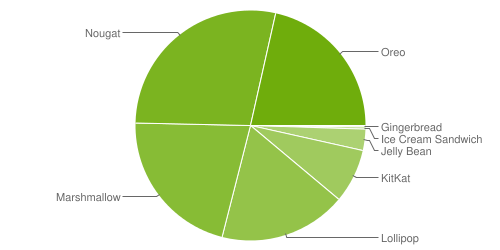
\includegraphics[width=0.7\textwidth]{obrazky-figures/market-share.png}
	\caption{Podiel verzií Androidu na trhu za rok 2018\protect\footnotemark. Poradie verzií od najnižšej je Gingerbread, Ice Cream Sandwich, Jelly Bean, KitKat, Lollipop, Marshmallow, Nougat, Oreo.}
	\label{market-share}
\end{figure}

\footnotetext{https://developer.android.com/about/dashboards}

Od verzie KitKat v Androide prebehlo mnoho zmien, uvedené budú len tie, ktoré sú zahrnuté v rámci tejto práce a bola zaistená ich spätná kompatibilita s verziou KitKat. 

\textbf{Material design} je jazyk pre tvorbu dizajnu vytvorený spoločnosťou Google. Predstavený bol prvýkrát vo verzii Androidu 5 a jeho hlavnou myšlienkou je poskytovať vysokokvalitné zobrazenie naprieč mnohými platformami, príjemne a jednoducho vyzerajúci vzhľad, ktorý kognitívne prepája elementy na obrazovke s tými reálnymi pre zníženie zaťaženie užívateľa a eliminuje nepredvídateľnosť, nejasnosť a chaos. Typické je rozloženie elementov do mriežky, responzívne animácie a prechody a rôzne vizuálne efekty. Tento dizajn je využitý aj v rámci grafického rozhrania aplikácie.

\textbf{Oprávnenia} aplikácií a ich prideľovanie sa zmenilo príchodom verzie Androidu 6. Oprávnenia sa už nemuseli prijať všetky naraz pri inštalácii aplikácie, naopak od tejto verzie ich užívateľ môže selektívne prijať alebo odmietnuť. Bližšie sú oba systémy oprávnení popísané v sekcii~\ref{permissions} o oprávneniach.

\subsubsection{Kompatibilita}

Každá aplikácia musí špecifikovať aké verzie Androidu podporuje. Táto skutočnosť je špecifikovaná v Gradle súbore alebo v manifeste. Spätná kompatibilita je silnou stránkou Androidu a preto sa pri vydaní novej verzie Androidu nemusia zvyčajne robiť veľké zásahy do kódu. Kompatibilitu určujú tri hlavné nastavenia -- \texttt{targetSdkVersion}, \texttt{minSdkVersion} a \texttt{compileSdkVersion}~\cite{Thornsby}.

\begin{itemize}

\item{\texttt{\textbf{minSdkVersion}} označuje najnižšiu verziu API (rozhranie pre programovanie aplikácie), na ktorej bude aplikácia fungovať.  Každá verzia Androidu so sebou nesie aj novú verziu API. Umožnenie inštalácie aplikácie na zariadenie je podmienené splnením požiadavky minimálnej verzie Androidu. Táto hodnota je dôležitá aj pri vývoji aplikácie, pretože sa v rámci projektu spúšťajú vlákna, ktoré majú za úlohu detekciu a upozornenie na využívanie funkcionality, ktorá je mimo dosah minimálnej verzie API. Ak by sa daná kontrola nediala, na nižších verziách Androidu by došlo k poruchám kvôli používaniu funkcií, ktoré ešte v danom API neexistujú. Všetky knižnice, ktoré aplikácia používa majú tiež vlastnú najnižšiu verziu API, ktorá by mala byť aspoň tak vysoká, ako najnižšia verzia API v aplikácii. Všeobecne sa táto hodnota nastavuje tak, aby pokrývala čo najväčšiu časť trhu. V rámci tejto práce sa používa minimálna verzia API 19, čo predstavuje Android 4.4 (KitKat).}

\item{\texttt{\textbf{targetSdkVersion}} označuje najvyššiu verziu API, na ktorej bude aplikácia plne funkčná. Prostredníctvom tohto nastavenia Android poskytuje kompatibilitu smerom dopredu. Novú funkcionalitu, ktorá je mimo dosah \texttt{targetSdkVersion} nepoužíva, až kým sa neaktualizuje hodnota tohto nastavenia. Táto hodnota by mala byť vždy nastavená na najvyššiu možnú, aby aplikácia mohla ťažiť z opráv a funkcionality uvedenej v novších verziách API. Aktualizácii hodnoty nastavenia by malo predchádzať dôkladné testovanie aplikácie, pretože úplná kompatibilita nie je zaručená. V rámci tejto práce sa používa najvyššia verzia API 28, čo predstavuje Android 8 (Pie).}

\item{\texttt{\textbf{compileSdkVersion}} určuje verziu API, pomocou ktorej sa aplikácia kompiluje. Kým predošlé dve nastavenia sú dôležité aj po vydaní aplikácie a konštantne ovplyvňujú jej beh, toto nastavenie je aplikované len v čase kompilácie aplikácie. Nie je nijak zahrnuté v konečnej skompilovanej aplikácii, ktorá je určená na distribúciu do zariadení. Verzia API, pomocou ktorej sa kompiluje aplikácia v rámci tejto práce je zhodné s nastavením najvyššej verzie API, na ktorej je aplikácia funkčná.}

\end{itemize}


\chapter{Implementácia}
\label{implementace}


Implementácia prebehla v dvoch súbežných častiach, serverová a klientská.
Server funguje na PHP 7.2 formou jednoduchého web-servera, ktorý má za úlohu správne zatriediť a spracovať požiadavky, ktoré sa mu doručia a odpovedať na ne. Poskytuje aj zároveň prehľad o jednotlivých pripojeniach a udržiava si aktuálny súbor s informáciami o pripojeniach. 

Klientská časť je Android aplikácia vyvíjaná v prostredí Android Studio\protect\footnotemark. Má za úlohu odosielať segmenty a logy na server, poskytovať jednoduché užívateľské rozhranie a koordinovať vlákna, ktoré sa podieľajú na odosielaní. V prípade výpadku internetového pripojenia musí zaistiť, aby sa segmenty nestrácali a udržali si svoju integritu. Je uspôsobená na dlhodobý a spoľahlivý beh.
\footnotetext{https://developer.android.com/studio/}


\section{Kódovanie nahrávky}

Výsledok nahrávania pomocou \texttt{AudioRecord} objektu predstavuje pole hodnôt (buffer) so šírkou 16 bitov nameraných zo zvukového zdroja. Obsah buffru tvorí jeden segment nahrávky, ktorý nie je možné poslať bez úpravy na server a to kvôli tomu, že PHP nepodporuje tento dátový typ. Nahrávky sú teda kódované pomocou base64. Base64 je kódovanie, ktoré prevádza binárne dáta do postupnosti znakov. Často sa používa na prenos binárnych dát kanálmi, ktoré podporujú len prenos textovou formou, čo je prípad komunikačného protokolu tejto aplikácie, pretože všetky odosielané údaje sú jednotného textového charakteru. Na serveri sa segment dekóduje a vzniká z neho ekvivalent bytového poľa, ale s použitím dátového typu reťazec. Tento dekódovaný reťazec sa následne už môže uložiť a prehrávať.

\section*{Typy buffrov}
Aplikácia rozlišuje medzi dvomi typmi buffrov: nahrávací a odosielací.

\textbf{Nahrávací buffer} slúži na ukladanie jednotlivých úsekov audia, ktoré sú zvyčajne veľmi krátke (v radách milisekúnd). Jeho veľkosť sa nedá určiť užívateľsky, ale vypočíta sa vždy po štarte aplikácie a zvolení konfigurácie audia. Veľkosti sa pri rovnakej konfigurácii môžu líšiť na základe modelu zariadenia alebo verzie operačného systému. Vypočíta sa pomocou funkcie obsiahnutej v Android SDK, ktorá na základe konfigurácie kanála, vzorkovacej frekvencie a bitovej hĺbky vypočíta minimálnu veľkosť buffru v bytoch, ktorá je potrebná pre nahrávanie. Tento buffer sa potom predá \texttt{AudioRecord} objektu a ten doň ukladá dáta prečítané z hardvéru.

\label{sending-buffer}
\textbf{Odosielací buffer} sa inicializuje s užívateľsky zvolenou veľkosťou, zvyčajne to sú veľkosti väčšieho charakteru. Udáva ako často sa budú odosielať dáta na server. Odosielací buffer musí byť menší ako nahrávací buffer, pretože vždy keď sa nahrajú vzorky do nahrávacieho buffru, tak sa pridajú na koniec odosielacieho buffru. Keď sa tento buffer naplní, jeho obsah sa odošle servera a následne sa vyprázdni.

\medskip
Pri implementácii sa ponúkala možnosť použitia iba jedného typu buffru, avšak obidva majú svoje opodstatnenie a použitie len jedného by spôsobilo problémy. Ak by odosielací buffer bol použitý na odosielanie, ale aj nahrávanie, nijako by to neovplyvnilo kvalitu nahrávky, avšak k analýze by sa  jednotlivé úseky audia dostávali menej často. To by znamenalo, že by nebola možná plynulá vizualizácia audia, ktorá je závislá na kontinuálnom toku vzoriek, z ktorých sa počíta vizualizovaná amplitúda. 

Naopak použitie iba nahrávacieho buffru by z technického hľadiska ničomu nebránilo, avšak výrazne by sa zvýšili požiadavky na zdroje a výkon u servera aj mobilného zariadenia. Malá veľkosť buffru by spôsobila, že požiadavky na server by prichádzali vo veľmi nízkych intervaloch a ak by sa odosielalo pomocou vlákien, zariadenie by mohlo byť zahltené množstvom vytvorených vlákien.

\newenvironment{pagebreakavoid}
  {\par\nobreak\vfil\penalty0\vfilneg
   \vtop\bgroup}
  {\par\xdef\tpd{\the\prevdepth}\egroup
   \prevdepth=\tpd}

\section{Moduly}


\begin{figure}[!hbt]
	\centering
	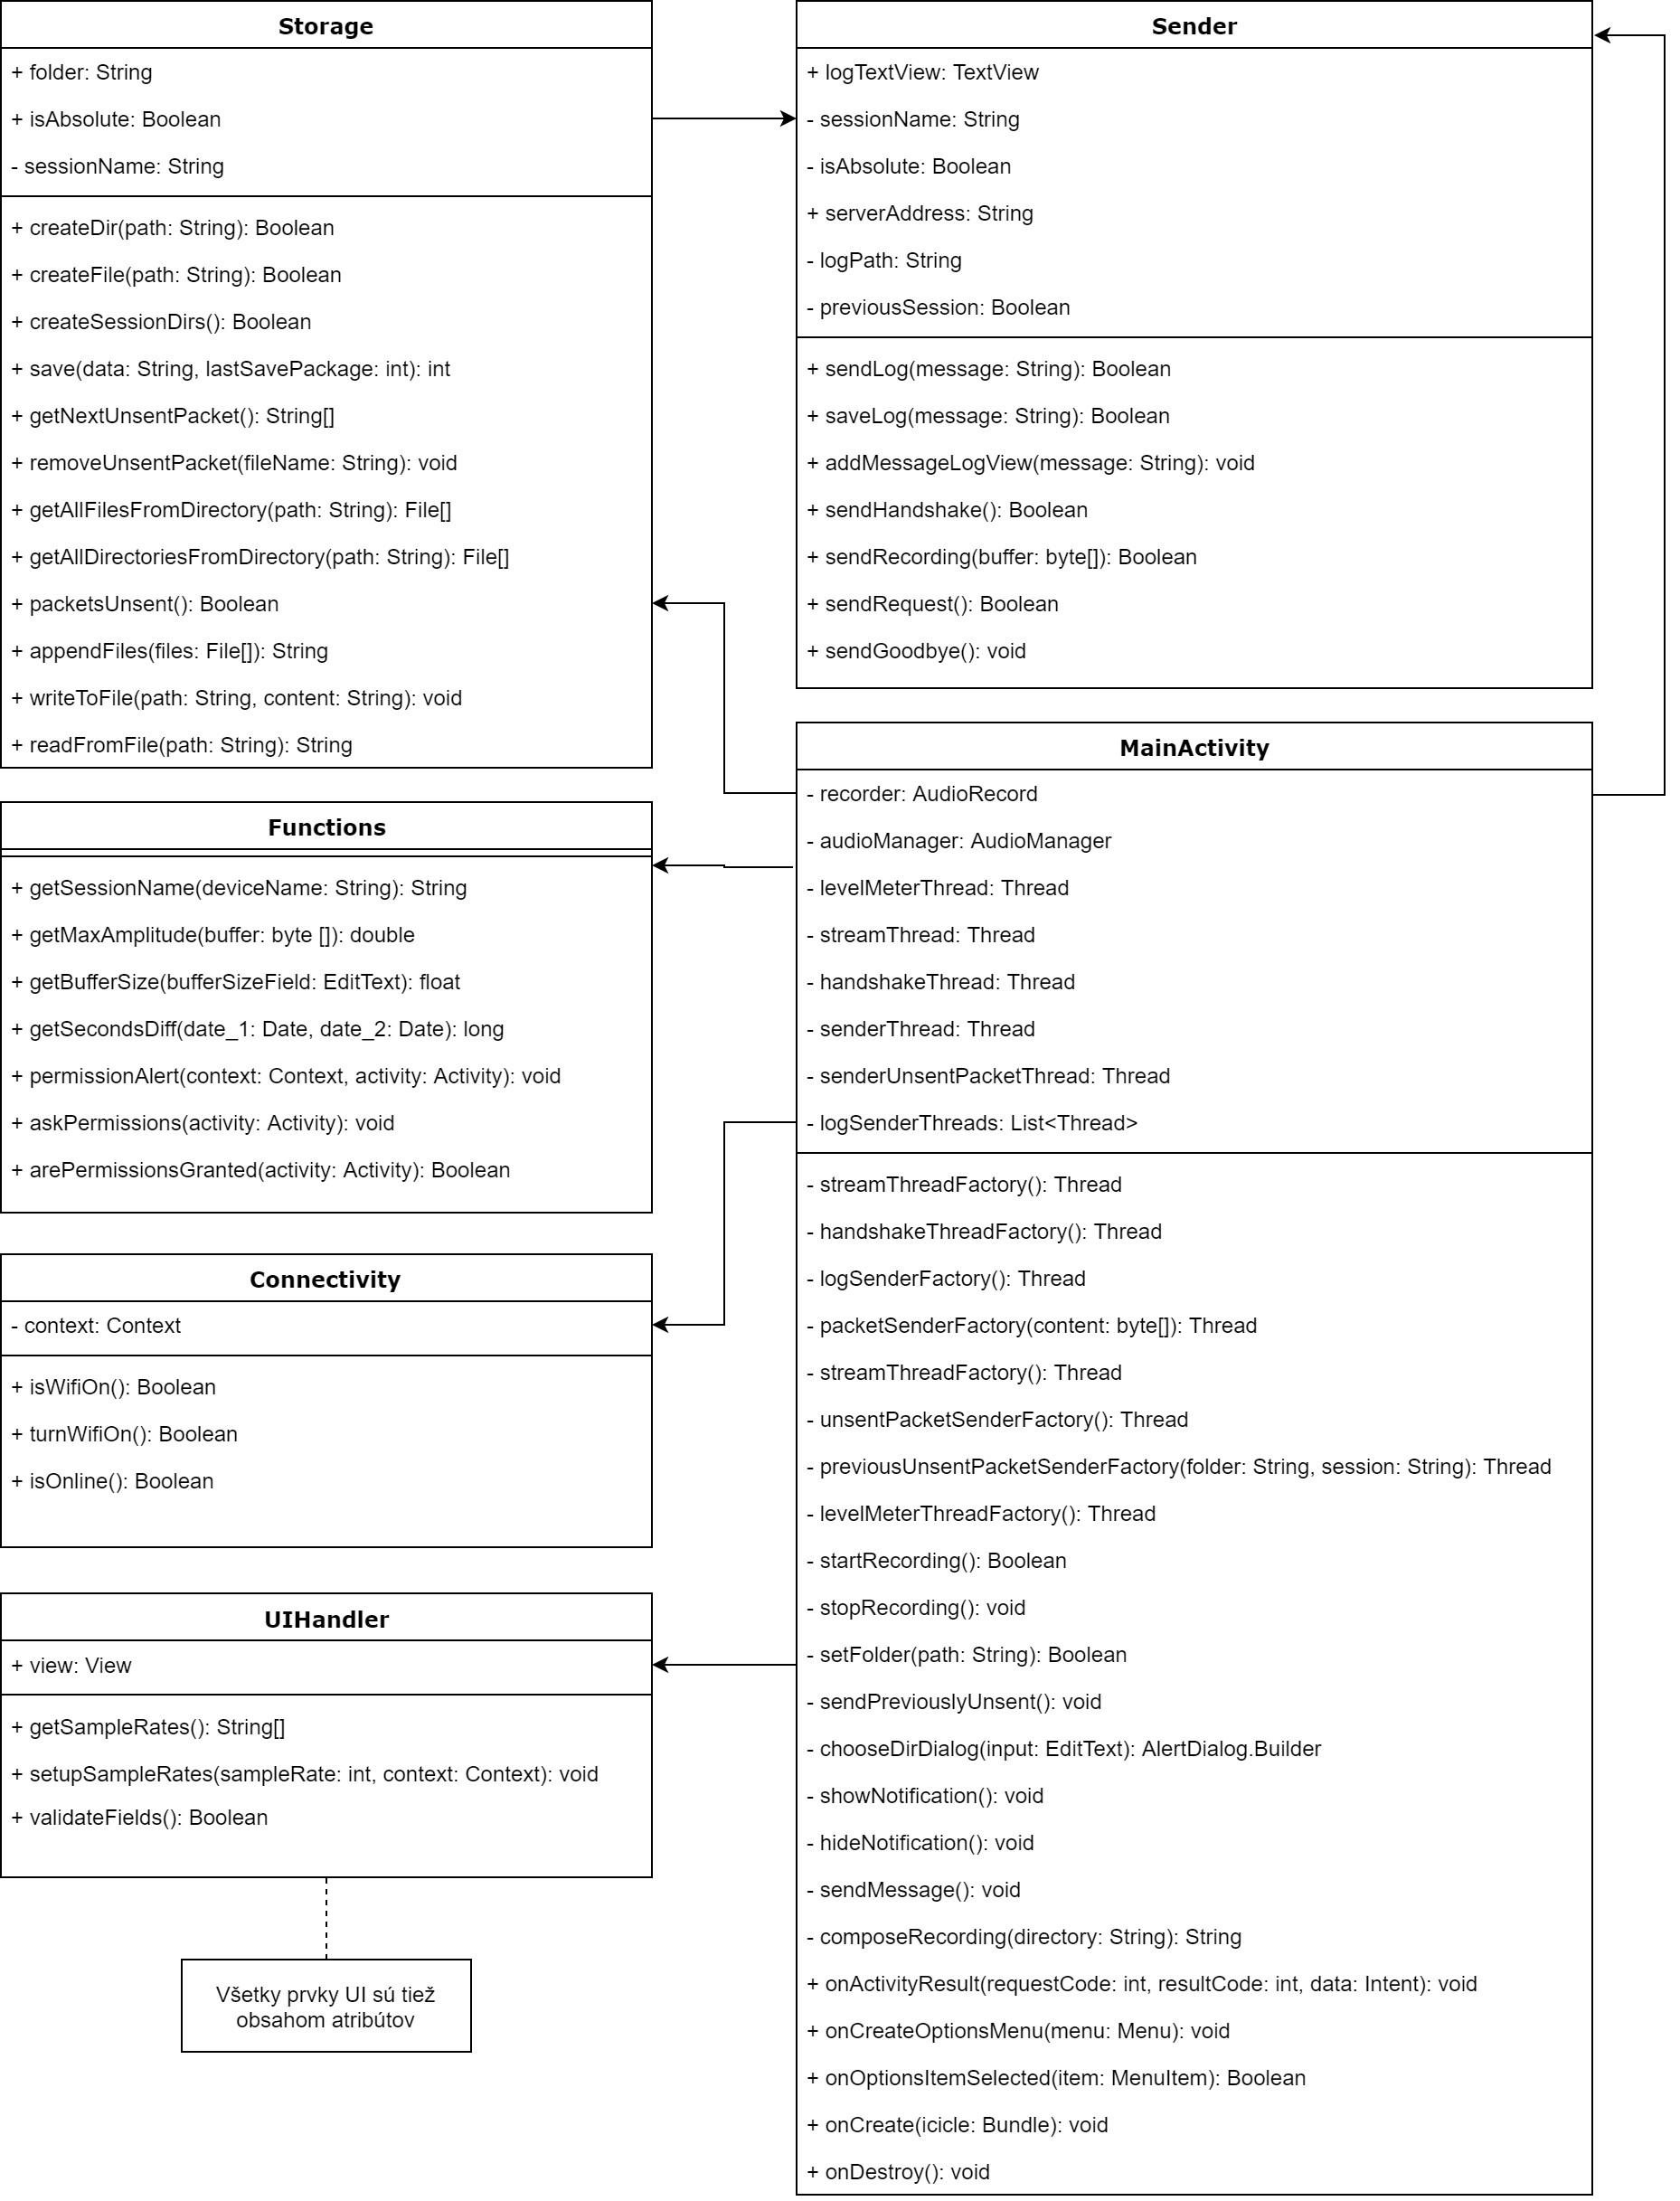
\includegraphics[width=1\textwidth]{obrazky-figures/class_diagram.png}
	\caption{Zjednodušený diagram tried.}
	\label{class_diagram}
\end{figure}

Aplikácia je rozdelená do samostatných modulov, kde každý z nich plní určitú skupinu účelov. Ilustrácia vzťahov, obsahu a využitia jednotlivých modulov je znázornená pomocou diagramu tried na obrázku~\ref{class_diagram}. Detailnejšie budú jednotlivé triedy popísané v nasledujúcej časti.

\subsection*{Storage}
Trieda Storage umožňuje manipuláciu s pamäťou zariadenia. Jej atribúty obsahujú primárne názov session a cesta k ukladacej zložke, avšak jej pôsobenie nie je obmedzené len na túto zložku. Obsahuje závislosť na triede \texttt{Sender} z dôvodu logovania pri poruchách. Jej metódy zahŕňajú:

\begin{itemize}
  \item{vytváranie zložiek potrebných pre každé nové nahrávanie,}
  \item{tvorbu nových súborov (logy, neodoslané segmenty),}
  \item{navigáciu neodoslanými segmentmi (ich detekcia, usporiadanie, získanie najstaršieho),}
  \item{rôzne pomocné metódy (čítanie/zápis do súborov, skladanie obsahu súborov, získanie všetkých zložiek/súborov zo zložky).}
\end{itemize}

\clearpage

\subsection*{Sender}

Komunikácia so serverom a logovanie je sprostredkované pomocou triedy \texttt{Sender}. Ten pre svoju funkciu potrebuje adresu servera (pre odosielanie požiadaviek), názov session, cestu k logu a widget pre zobrazovanie klientského logu v aplikácii. Každý záznam do logu, ktorý sa odošle na server sa uloží aj do klientského logu. Naopak to však už neplatí. \texttt{Sender} spĺňa nasledujúce funkcie:
   
   
\begin{itemize}
 \item{odosielanie logov na server,}
 \item{ukladanie logov lokálne,}
 \item{dopĺňanie obsahu klientského logu do widgetu v aplikácii a zabezpečenie posúvania na aktuálny log,}
 \item{odosielanie segmentov,}
 \item{odosielanie správ,}
 \item{úvodný handshake,}
 \item{ukončenie nahrávania s odoslaním klientského logu.}
\end{itemize}

\subsection*{Functions, Connectivity, UIHandler}

Trieda \texttt{Functions} obsahuje generické pomocné funkcie používané z akéhokoľvek iného modulu. Zaisťuje primárne:

\begin{itemize}
 \item{výpočet maximálnej amplitúdy,}
 \item{tvorbu identifikátoru session,}
 \item{získanie minimálnej veľkosti nahrávacieho buffru,}
 \item{žiadanie oprávnení,}
 \item{detekciu oprávnení,}
 \item{upozornenie užívateľa na chýbajúce oprávnenie.}
\end{itemize}

\label{connectivity}
Trieda \texttt{Connectivity} obsahuje metódy spojené s internetovým pripojením, ako napríklad:
\begin{itemize}
 \item{stav pripojenia k internetu,}
 \item{manipulácia s Wi-Fi pripojením.}
\end{itemize}
Pri zisťovaní internetového pripojenia neberie do úvahy len pripojenie pomocou Wi-Fi, testuje sa všeobecné pripojenie pomocou ľubovoľného prvku.

Obalenie prvkov užívateľského rozhrania zabezpečuje trieda \texttt{UIHandler}. V jej atribútoch sa nachádzajú všetky tlačidlá, polia a komponenty rozhrania, s ktorými manipuluje. Na začiatku aplikácie inicializuje rozhranie a doplní každému prvku príslušnú počiatočnú hodnotu a naplní hodnotami prvky, ktoré obsahujú množinu elementov (napríklad výber vzorkovacej frekvencie). Pred štartom každého nahrávania sa hodnoty všetkých prvkov validujú pomocou tejto triedy. 

\subsection*{MainActivity}

Jadro aplikácie a najdôležitejšia trieda, ktorá využíva všetky ostatné. Spúšťa sa prostredníctvom nej celá aplikácia a ovláda spracovanie užívateľského vstupu. Obsahuje mnoho atribútov (nastavenia nahrávania, názov session a zariadenia, status nahrávania, atď.), avšak najvýznamnejšie zahŕňajú \texttt{AudioRecord} objekt (pomocou neho prebieha celé nahrávanie), \texttt{AudioManager} objekt (nahrávanie prostredníctvom Bluetooth) a atribúty pre dva hlavné vlákna (nahrávacie vlákno a vlákno pre meranie úrovne audia), pričom v jeden konkrétny moment beží len jedno z nich.

Nahrávacie vlákno zahŕňa aj meranie úrovne audia, ale je to jeho interný proces. V stave nečinnosti aplikácie (neprebieha nahrávanie) je spustené vlákno na meranie úrovne audia, ktorého jediným účelom je periodická aktualizácia hodnoty úrovne, ktorá sa využíva na vizualizáciu audia. Keďže tieto vlákna by nemali byť spustené naraz, ukladajú sa do atribútov.

Veľká časť aktivity aplikácie prebieha vo vláknach, ktoré trieda \texttt{MainActivity} tvorí, spúšťa, prerušuje v prípade potreby a stará sa o to, aby sa vzájomne nijak negatívne neovplyvňovali. Obsahuje 6 metód pre tvorbu vlákien.
\begin{itemize}
 \item{\texttt{\textbf{packetSenderFactory}} tvorí odosielacie vlákno pre segmenty z aktuálne prebiehajúceho nahrávania, ktoré je charakteristické krátkou životnosťou a v jeden okamih môže bežať len jedna inštancia tohto vlákna. Jeho primárnym cieľom je doručiť segment nahrávky na server. V prípade zlyhania sa segment ukladá do úložiska a aktualizuje sa stav aplikácie na offline. Neodoslané segmenty sa do pamäte zariadenia ukladajú ako textové súbory obsahujúce segment vo forme reťazca zakódovaného pomocou base64. Názov súboru označuje zároveň aj poradie segmentu.}

 \item{\texttt{\textbf{unsentPacketSenderFactory}} tvorí odosielacie vlákno pre neodoslané segmenty nahrávky v rámci bežiaceho nahrávania. Pracuje s aktuálnou session, takže sa môže vytvoriť a spustiť iba ak je nahrávanie aktívne a prebehla úvodná požiadavka na server. Stará sa o odoslanie všetkých segmentov, ktoré sa nachádzajú v úložisku zariadenia a pokiaľ je aktívne, nijaké segmenty sa neodosielajú pomocou odosielacieho vlákna pre segmenty z aktuálneho nahrávania, ale ukladajú sa do úložiska. V jeden okamih môže bežať iba jedno vlákno tohto typu a končí svoju prácu vyprázdnením neodoslaných segmentov pre danú session. V prípade zastavenia nahrávania sa vlákno preruší. Vlákno pre odosielanie neodoslaných segmentov nemôže bežať zároveň s vláknom pre odosielanie aktuálne nahraných segmentov. Pri úspešnom odoslaní segmentu aktualizuje stav aplikácie na online. Pri neúspešnom odoslaní sa pokúsi zapnúť internetové pripojenie.}
 
  \item{\texttt{\textbf{handshakeThreadFactory}} slúži na vytváranie handshake požiadaviek. Handshake musí prebehnúť predtým než sa k danej session na server uloží akýkoľvek log alebo záznam. V jeden moment môže bežať len jedna inštancia tohto vlákna, aby nedošlo k prípadom, kde sa server zahltí handshake požiadavkami. Toto vlákno sa vytvára vždy na začiatku nahrávania a pri neúspechu sa potom môžu jeho vytvorenie zopakovať pred pokusom o odoslanie segmentu na server.}


    \item{\texttt{\textbf{logSenderFactory}} zabezpečuje odosielanie logov. Tomu predchádza uloženie do klientského logu pre zachovanie čo najväčšej podobnosti serverového a klientského logu. Po uložení do klientského logu sa pokúsi odoslať log na server. Pri neúspechu však nevykoná nijakú akciu, log sa už nepokúša opätovane odoslať. Vlákien pre odoslanie logov môže byť ľubovoľné množstvo a majú veľmi krátku životnosť, najdlhšia možná je súčtom maximálneho časového limitu pre odoslanie logu na server a doby pre uloženie logu lokálne a pri neúspešnom odoslaní logu ho na rozdiel od vlákien pre odoslanie segmentov už nikam neukladajú. Preto nemôže dôjsť k zahlteniu klienta týmito vláknami. Pri pomalšom pripojení však hrozí, že pokiaľ beží v jednom momente viacero týchto vlákien, môžu odoslať svoje logy na server v zlom poradí. Práve preto sa všetky vlákna tohto typu ukladajú do zoznamu a vždy môže v jednu dobu odosielať len vlákno, ktoré je na čele zoznamu. Po ukončení činnosti sa zo zoznamu odstráni a predáva činnosť ďalšiemu vláknu. V prípade absencie handshake požiadavky pre danú session logy iba ukladajú lokálne.}

 \item{\texttt{\textbf{streamThreadFactory}} tvorí hlavné nahrávacie vlákno, ktoré riadi odosielanie a ukladanie segmentov a chod aplikácie. Podľa potreby volá jednotlivo predchádzajúce dva vlákna za účelom odoslania nahrávok na server. Taktiež sa stará o pravidelnú aktualizáciu úrovne audia a prostredníctvom triedy \texttt{Connectivity}~\ref{connectivity} zaisťuje pripojenie, prípadne vkladá do logu problémy s pripojením.}

 \item{\texttt{\textbf{levelMeterThreadFactory}} tvorí vlákno pre meranie úrovne audia. Beží vždy, keď je nahrávanie neaktívne.}

 \item{\texttt{\textbf{previousUnsentPacketSenderFactory}} tvorí vlákno pre spätné odoslanie neodoslaných segmentov v rámci jednej skončenej session, ktorej zložku kontroluje na prítomnosť neodoslaných segmentov. Má stredne dlhú životnosť a v jeden okamih môže bežať viacero vlákien tohto typu a nijak neovplyvňujú nahrávanie. Pri strate pripojenia alebo neúspechu odoslania toto vlákno nečaká v cykle na pripojenie, ale uloží túto skutočnosť do logu a končí svoju činnosť. Ak ostali nejaké segmenty, odošlú sa pri najbližšom hľadaní neodoslaných segmentov z ukončených sessions novým vláknom. }
\end{itemize}

Medzi funkcie, ktoré plní \texttt{MainActivity} patrí:
\begin{itemize}
 \item{inicializácia aplikácie,}
 \item{riadenie činnosti aplikácie pomocou vlákien a modulov,}
 \item{informovanie o činnosti aplikácie,}
 \item{spravovanie notifikácií,}
 \item{kompozícia nahrávok,}
 \item{riadenie menu,}
 \item{riadenie komponentov pre prehliadanie úložiska zariadenia a spracovanie ich výstupov.}
\end{itemize}

Táto trieda nie je používaná žiadnymi inými, preto sú všetky jej atribúty a takmer všetky metódy nastavené ako privátne. Výnimkou sú metódy, ktoré sú definované v rodičovskej triede \texttt{MainActivity}, ktorá sa nazýva \texttt{AppCompatActivity}. \texttt{AppCompatActivity} dedí z \texttt{Activity}, ktorá predstavuje jednu obrazovku s užívateľským rozhraním, bude sa označovať názvom aktivita. Aktivita načíta všetky vizuálne komponenty a každá aplikácia môže mať viacero aktivít a každá musí byť definovaná v manifeste. Aktivita má definovaný životný cyklus, ktorý je znázornený na obrázku~\ref{activity}.


Každá aktivita v rámci aplikácie môže redefinovať chovanie metód, ktoré sú súčasťou jej životného cyklu. \texttt{MainActivity} redefinuje chovanie pri jej vytvorení a zániku. Pri vytvorení \texttt{MainActivity} sa volá metóda \texttt{onCreate}, ktorá nastaví začiatočné hodnoty prvkov užívateľského rozhrania a spustí vlákno pre meranie úrovne audia. Taktiež pre každú časť užívateľského rozhrania od ktorej sa požaduje pri konkrétnej akcii isté chovanie definuje funkciu, ktorá sa zavolá, keď nastane daná akcia (napríklad otvorenie prehliadača zložiek pri aktivácii tlačidla pre zmenu ukladacej zložky). Aktivita môže byť prerušená dvomi spôsobmi. Pri stlačení spätného tlačidla na zariadení alebo pri ukončení aplikácie systémom sa zavolá metóda \texttt{onDestroy}, ktorá v \texttt{MainActivity} uvoľní všetky zdroje a ak bežia nejaké vlákna, tak ich ukončí. Ak by neboli ukončené, aplikácia by uvoľnila aktivitu, avšak vlákna by ostali voľne bežať bez akejkoľvek referencie na nich a zaberali by zdroje na nahrávanie audia, čo by znemožňovalo prácu aplikácii pri opätovnom štarte. Ak užívateľ stlačí domovské tlačidlo na zariadení, aktivita sa neuvoľní, ale beží stále na pozadí a dá sa do nej vrátiť.

\begin{figure}[!hbt]
	\centering
	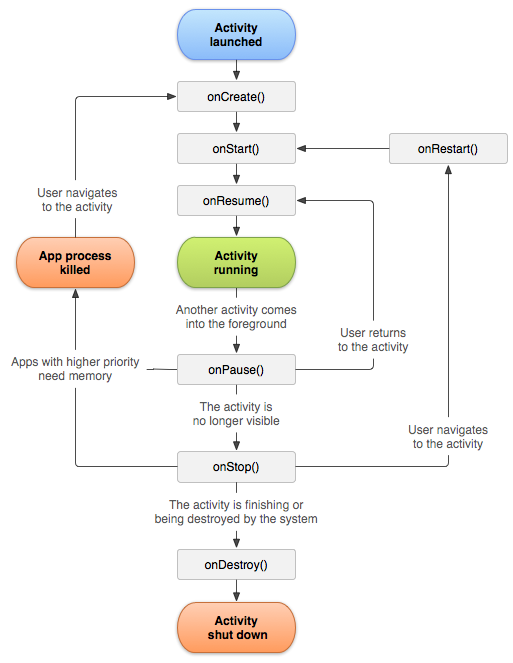
\includegraphics[width=0.7\textwidth]{obrazky-figures/activity.png}
	\caption{Životný cyklus Android aktivity\protect\footnotemark.}
	\label{activity}
\end{figure}
\footnotetext{https://developer.android.com/guide/components/activities/activity-lifecycle}

\pagebreak

\section{Užívateľské rozhranie}

Vzhľad aplikácie je minimalistický, dôraz bol kladený na prehľadné užívateľské rozhranie, ktoré obsahuje len základné riadiace prvky dôležité pre chod aplikácie a zároveň umožňuje nastavenie všetkých požadovaných funkcií. Rozhranie je znázornené na obrázku~\ref{ui}.

\begin{figure}[hbt]
	\centering
	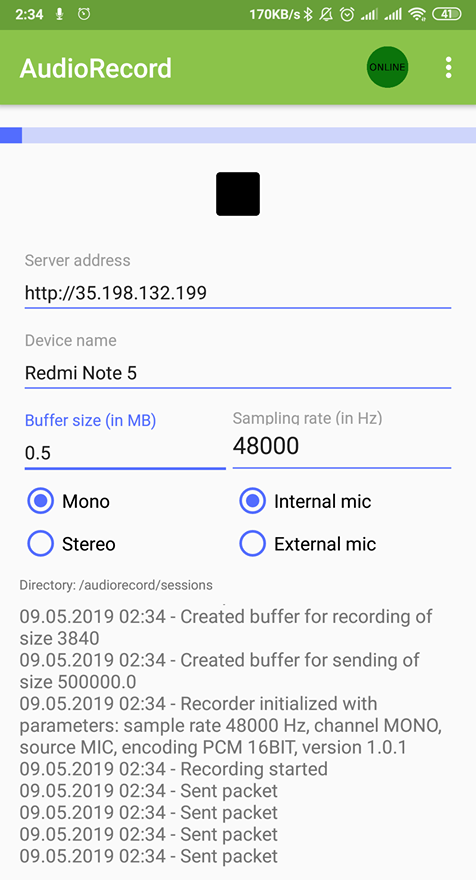
\includegraphics[width=0.5\textwidth]{obrazky-figures/ui.png}
	\caption{Vzhľad aplikácie počas nahrávania. V hornej lište sa nachádza ikona notifikácie pre nahrávanie.}
	\label{ui}
\end{figure}

\begin{figure}[hbt]
	\centering
	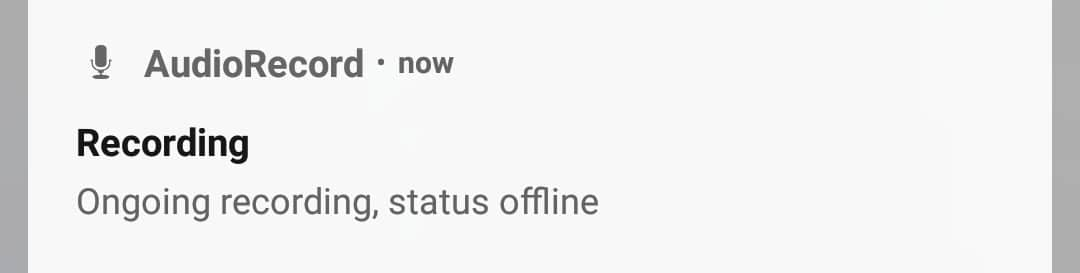
\includegraphics[width=0.5\textwidth]{obrazky-figures/notification.png}
	\caption{Ukážka notifikácie pri offline nahrávaní.}
	\label{notification}
\end{figure}

\begin{figure}[hbt]
	\centering
	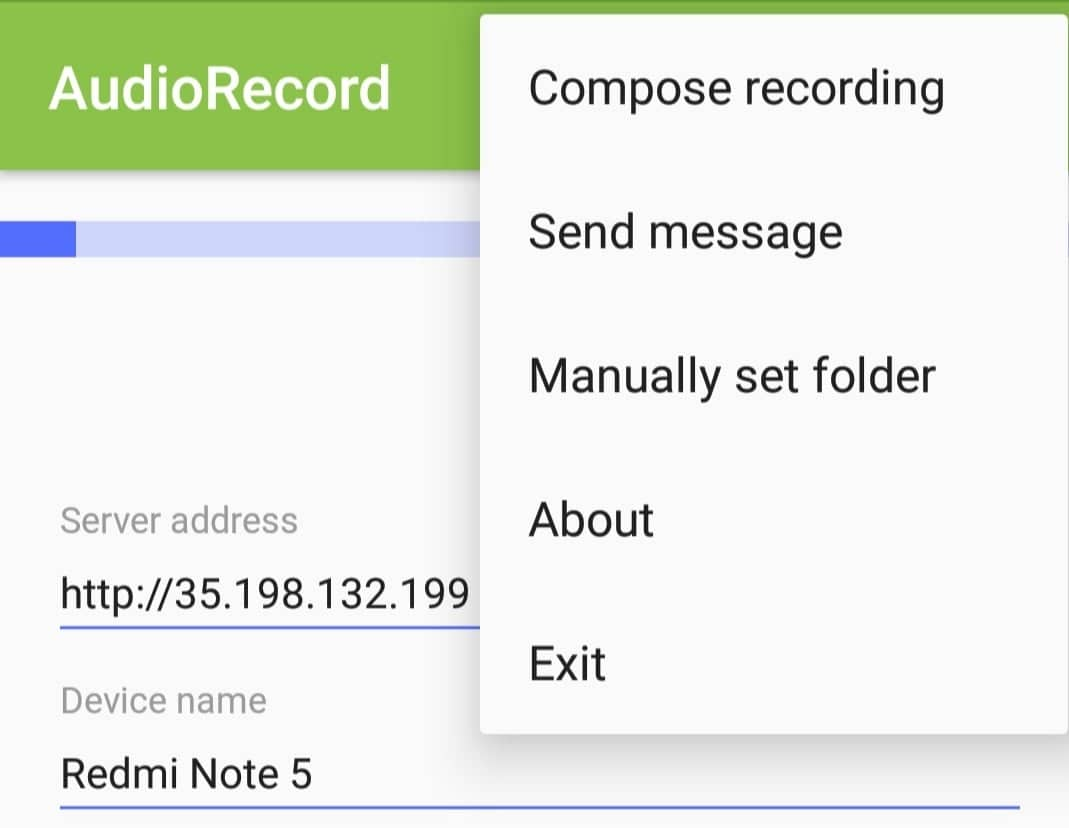
\includegraphics[width=0.5\textwidth]{obrazky-figures/ui-menu.png}
	\caption{Menu aplikácie.}
	\label{ui-menu}
\end{figure}

\begin{figure}[hbt]
	\centering
	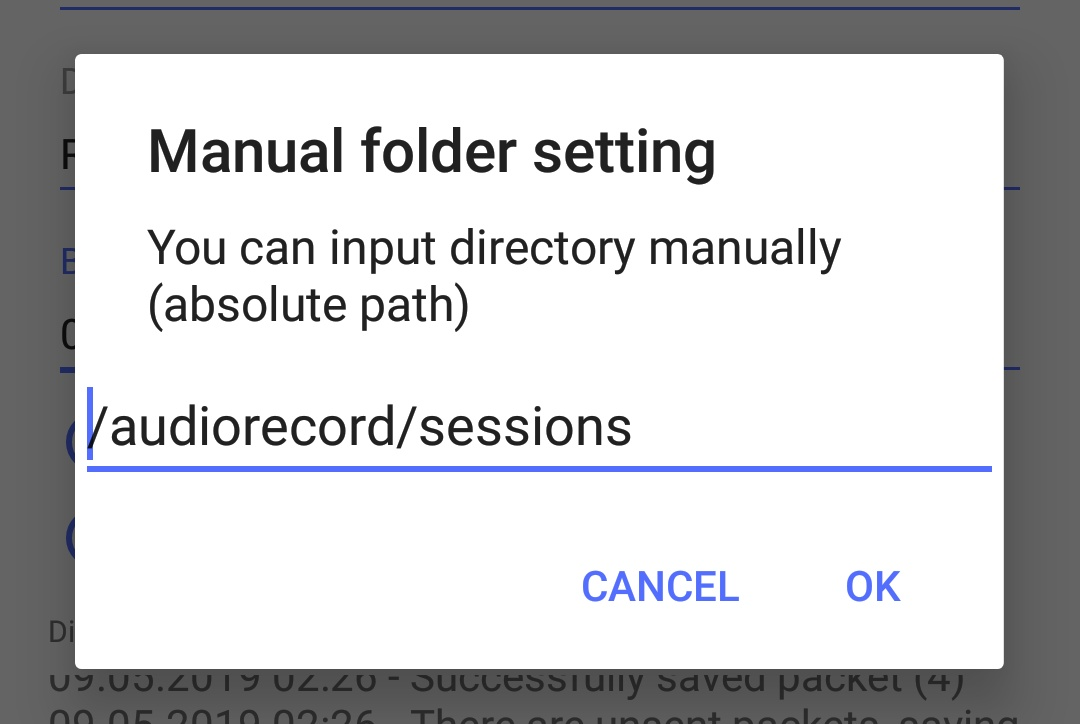
\includegraphics[width=0.5\textwidth]{obrazky-figures/ui-directory-chooser.png}
	\caption{Okno pre manuálne zadanie cesty úložiska pri absencii prehliadača zložiek.}
	\label{ui-directory-chooser}
\end{figure}

Menu, ktoré obsahuje informácie o aplikácii, možnosť odoslania vlastnej správy na server, ukončenie aplikácie, manuálne zvolenie úložiska a možnosť kompozície nahrávky bez prítomnosti servera sa nachádza v pravom hornom rohu a jeho obsah je znázornený na obrázku~\ref{ui-menu}. Súčasťou aplikácie je aj notifikácia, ktorá sa zobrazuje počas celého nahrávania a je perzistentná (nie je možné ju klasicky zrušiť potiahnutím) a je znázornená na obrázku~\ref{notification}. Bol kladený dôraz na to, aby všetky frekventované nastavenia boli viditeľné konštantne v rozhraní aplikácie a neboli schované v menu. Možnosť odoslania vlastnej správy dáva užívateľovi priestor si do nahrávania vkladať vlastné poznámky alebo identifikátory príslušné k danej session, zariadeniu alebo časovom údaji v rámci nahrávania. Tieto správy sa uložia do klientského aj serverového logu a zobrazia sa aj v dolej časti aplikácie pre prehľad logov. Správu je možné odoslať len počas nahrávania. Pri absencii internetového pripojenia sa správa ukladá len do klientského logu, užívateľ je však o tom informovaný. Tlačidlo pre ukončenie aplikácie uvoľní všetky zdroje, ukončí všetky vlákna, zruší notifikáciu a bezpečne zavrie aplikáciu. Pokiaľ je nahrávanie aktívne v čase ukončenia, pošle sa serveru požiadavka o ukončení session a až potom sa aplikácia zavrie.

Vedľa menu sa nachádza indikátor spojenia so serverom. Červená farba značí stav nepripojenia a zelená farba značí aktívne pripojenie. Stav indikátora sa mení len v rámci nahrávania, kde pri neúspešnej požiadavke sa zároveň mení stav indikátora a každá úspešná požiadavka môže spôsobiť prechod do aktívneho stavu, pokiaľ je aktuálny stav opačný. Zmena indikátora sa dosiahne prekreslením menu, ktoré zahŕňa aj prekreslenie notifikácie. 

V hornej časti rozhrania je bledomodrý pás, ktorý slúži na vizualizáciu nahraného audia. Počíta sa ako maximálna amplitúda z krátkych úsekov audia a jeho aktivita sa dá popísať ako neustále rastúci alebo klesajúci ukazovateľ postupu. Hneď pod ním je tlačidlo na ovládanie nahrávania zvuku, ktoré sa mení na základe momentálne prebiehajúcej činnosti a to buď na tlačidlo pre spustenie nahrávania alebo tlačidlo pre zastavenie nahrávania.

Nasleduje nastavenie adresy servera, na ktorý sa budú dáta posielať. Server si dané zariadenie potrebuje špecificky označiť (a dané značenie by malo byť aj zrozumiteľné) a na to sa využíva názov zariadenia. Môže byť pri každom nahrávaní identické, pretože kompletný identifikátor zariadenia na serveri zahŕňa aj časový údaj. Nastavenie buffru je číselný údaj a konkrétne označuje nastavenie odosielacieho buffru. Ďalšími dôležitými prvkami sú nastavenie konfigurácie kanálu a vzorkovacej frekvencie. Výber vzorkovacej frekvencie je riešený zvolením z hodnôt. Zahrnuté sú všetky rozšírené hodnoty, na ktoré sa v inicializačnej časti aplikácie jednotlivo vykonáva testovanie podpory zariadením a až vtedy sa zaradia do zoznamu možností, z ktorých sa dá vybrať. Nastavenie zdroja nahrávaného zvuku môže byť interné (interný mikrofón, káblom pripojený mikrofón) alebo externé (bezdrôtový mikrofón).

Keďže sa na zariadenie budú ukladať logy a poprípade aj úseky nahrávania, ktoré sa neodoslali na server, je potrebné zvoliť cestu k ukladacej zložke. Pod konfiguráciu všeobecných nastavení zvuku a nahrávania sa nachádza cesta k zložke, kam sa budú ukladať dáta spojené s chodom aplikácie. Po dotyku tejto možnosti sa otvorí prehliadač súborov, ktorý umožní zvoliť zložku na ukladanie. Na začiatku sa automaticky zvolí štandardná zložka, ktorá je umiestnená v koreni úložiska.

Pri voľbe zložky však môžu nastať problémy. Kým väčšina zariadení má v sebe zabudovaný prehliadač súborov, nie každé z nich má prehliadač zložiek. Pokiaľ zariadenie prehliadač zložiek obsahuje, niekedy môže zahŕňať len prehliadanie interného úložiska a na pamäťovú kartu sa už nedostane. Pre umožnenie výberu úložiska bez ohľadu na to, či sa nachádza v internej alebo externej pamäti, je v aplikácii možnosť manuálneho nastavenia úložiska zadaním absolútnej cesty k priečinku textovou formou. Toto riešenie zabezpečuje možnosť zmeny úložiska bez potreby inštalácie prehliadača zložiek. Po detekcií programov pre prehliadanie zložiek môže nastať, že zoznam program je prázdny. Zobrazí sa dialógové okno (viď. obrázok~\ref{ui-directory-chooser}), ktoré oznamuje absenciu prehliadača súborov a zároveň užívateľovi ponúka možnosť manuálneho zadania cesty k zložke. Toto okno je možné zrušiť alebo zadať cestu, pri ktorej sa následne kontroluje to, či je to skutočne adresár a či existuje. Pokiaľ existuje prehliadač zložiek, užívateľ má stále možnosť manuálneho nastavenia zložky pomocou voľby v hornom menu. Zadaná cesta musí byť vždy absolútna.

V spodnej časti sa nachádza okno, ktoré informuje užívateľa o momentálnej činnosti nahrávania. Zobrazuje sa v ňom všetko, čo sa uloží do logu na klientovi. Oknom sa dá posúvať a zobrazovať si tak udalosti v minulosti. Pri pridaní novej informácie do tohto okna sa jeho obsah automaticky posunie tak, aby bola informácia viditeľná, takže sa priebeh nahrávania dá sledovať bez akejkoľvek akcie naviac.

Celá validácia obsahu nastavení a overenie toho, či je nahrávanie pod danou konfiguráciou možné nastáva až pred spustením nahrávania. V prípade chyby sa nesprávna alebo chýbajúca hodnota patrične zvýrazní. Musia sa špecifikovať všetky nastavenia.

\subsubsection{Ukladanie nastavení}

Zmeny vykonané v užívateľskom rozhraní sú stáleho a obsiahleho charakteru (adresa servera bude väčšinou rovnaká pre každé nahrávanie), preto je vhodné niektoré konfiguračné nastavenia lokálne ukladať a pri opätovnom štarte aplikácie nastaviť začiatočnú hodnotu prvkov z uložených hodnôt. V aplikácii prebieha ukladanie zložky pre nahrané dáta, adresy servera a názvu zariadenia. Tieto konfiguračné nastavenia sa ukladajú pomocou objektu \texttt{SharedPreferences} (zdieľané preferencie). Táto trieda umožňuje ukladať dáta na princípe kľúč a hodnota. Hodnoty sa zapisujú cez editor, ktorý je súčasťou triedy \texttt{SharedPreferences}. Hodnoty sa ukladajú do automaticky vytvoreného XML súboru v internom úložisku zariadenia. Pri odstránení aplikácie zo zariadenia sa odstránia aj jeho preferencie.

\subsubsection{Audio level meter}

Ako už bolo znázornené na obrázku~\ref{ui}, jednou z funkcií užívateľského rozhrania je zobrazovanie úrovne audia. Aplikácia úrovne zobrazuje hneď po jej štarte. Proces zachytávania audia pre vizualizáciu sa však líši pre stav aktívny stav (nahrávanie a odosielanie na server) a stav nečinnosti.

Pri štarte aplikácie sa vytvorí vlákno, ktoré pomocou \texttt{AudioRecord} objektu zaznamenáva zvuk a na základe neho mení vizualizáciu úrovne audia. Zaznamenané audio sa nijako neukladá ani nespracúva, vypočíta sa z neho iba úroveň pre vizualizáciu. Je rozdelené na menšie segmenty, ktoré sú tvorené číselnými hodnotami o veľkosti 16 bitov. Hodnoty sa prevedú na absolútne a z nich sa získa maximum, ktoré sa potom zobrazí ako úroveň audia. Prvok pre zobrazenie úrovne audia má maximálnu hodnotu 100, takže hodnota amplitúdy sa mapuje do 0 do tejto hodnoty.

 Toto vlákno beží len v prípade, že neprebieha nahrávanie a to z toho dôvodu, že táto aktivita potrebuje iný druh vlákna, ktorý audio po nahraní a nastavení vizualizácie nezahodí, ale ďalej ho spracúva (napríklad odoslaním na server). V prípade inicializácie nahrávania aktiváciou tlačidla pre ovládanie nahrávania, sa toto vlákno zruší. Pri zastavení nahrávania sa vlákno opätovne vytvorí a spustí, takto je zabezpečené, aby vizualizácia audia bola nepretržitá.

Zdroj zvuku pri meraní sa líši na základe situácie. Priamo po štarte začiatočné vlákno používa zvuk z interného mikrofónu. Pri zvolení možnosti nahrávania z externého mikrofónu sa však pri započatí nahrávania aj toto vlákno prepne a zobrazuje úroveň audia z externého zdroja. 

\section{Bluetooth nahrávanie}
\label{external-recording}


Okrem nahrávania cez interný mikrofón je možné nahrávať aj pomocou bezdrôtového mikrofónu. Toto nahrávanie je označené ako externé nahrávanie, poprípade nahrávanie externým mikrofónom. Primárne je dôraz kladený na nahrávanie pomocou Bluetooth headsetu. Všeobecné fungovanie Bluetooth v Androide je popísané v sekcii~\ref{bluetooth}. Táto časť bližšie vysvetlí konkrétnu implementáciu Bluetooth pripojenia a prenosu dát špecifickú pre aplikáciu. 

Po úvodných kontrolách (podpora Bluetooth na danom zariadení, overenie zapnutia funkcie Bluetooth) nasleduje detekcia dvoch dôležitých premenných. V užívateľskom rozhraní sa skontroluje stav výberu mikrofónu. Pomocou Bluetooth adaptéra sa potom v zozname rozpoznaných zariadení zisťuje prítomnosť akéhokoľvek headsetu a kontroluje sa, či je zariadenie pripojené. 

Ak je zvolená možnosť nahrávania interným mikrofónom, nezáleží na tom, či je headset pripojený alebo nie, pokračuje sa vytvorením nahrávacieho vlákna a používa sa interný mikrofón. Ak je však zvolená možnosť nahrávania externým mikrofónom, informácia o pripojení headsetu sa kontroluje. V prípade, že headset nie je pripojený, vypíše sa na obrazovku chybová hláška o absencii pripojeného externého mikrofónu a nahrávanie nezačne. Pokiaľ je externý mikrofón pripojený, vytvorí sa inštancia triedy \texttt{IntentFilter}. Intent je objekt pre odosielanie správ, ktorý je možné použiť na vyžiadanie akcie z iného komponentu aplikácie\protect\footnotemark. Tri hlavné prípady použitia zahŕňajú napríklad spustenie aktivity, služby alebo doručenie vysielania. Pre príjem dát pomocou Bluetooth bude použitý posledný prípad.
\footnotetext{https://developer.android.com/reference/android/content/Intent}

V objekte \texttt{IntentFilter} sa špecifikuje typ intentu na objekt, ktorý reaguje na zmeny stavu Bluetooth SCO pripojenia. Následne sa vytvorí inštancia triedy \texttt{BroadcastReceiver}, ktorý je hlavným aktérom príjmu dat z Bluetooth a pridelí sa objektu \texttt{IntentFilter}. \texttt{BroadcastReceiver} po štarte overí SCO pripojenie a spustí v rámci neho nahrávacie vlákno, ktoré už postupuje podobne ako pri nahrávaní interným mikrofónom. Toto zabezpečí, že akékoľvek nahrávanie bude realizované iba pomocou externého mikrofónu. Pri odpojení externého mikrofónu počas nahrávania sa nahrávanie preruší.


\section{Server}

Server má za úlohu prijímať segmenty nahrávky odosielané od klienta, správne ich uložiť a vytvárať prehľad o jednotlivých pripojeniach a ich štatistikách. Skladá sa z hlavého serverového súboru, ktorý sa spustí vždy, keď príde nová požiadavka a statickej stránky, ktorá slúži ako prehľad pripojení. Dôvodom minimalistického dizajnu servera a nepoužitie databázy na ukladanie nahrávok je odvodený z prípadu použitia aplikácie, kde nie je požadovaný komplexný server. 


\subsection*{Dashboard}

Dashboard je miesto, ktoré poskytuje zrozumiteľný a rýchly náhľad dôležitých informácií. Na serveri je definovaný pomocou HTML a PHP v osobitnom súbore. Poskytuje prehľad pripojeniach, ktoré môžu byť:
\begin{itemize}
  \item{aktívne -- server prijal a úspešne uložil aspoň jeden segment z tohto spojenia v časovom intervale posledných 5 minút,}
  \item{neaktívne -- server od tohto spojenia už aspoň 5 minút segment neprijal, avšak neprišla správa o ukončení nahrávania,}
  \item{ukončené -- toto spojenie bolo zastavené zo strany klienta.}
\end{itemize}
Dashboard uvádza aj čas príchodu posledného záznamu a údaj o tom, ako veľmi v minulosti sa tento čas nachádza. Pre účel kontroly korektnosti nahrávania poskytuje dashboard stiahnutie posledného prijatého záznamu. Tento záznam je k dispozícii len vtedy, keď nahrávanie prebehlo aspoň s čiastočnou účasťou servera. K dispozícii sú k nahliadnutiu alebo stiahnutie aj jednotlivé logy, pričom serverový log je k dispozícii neustále, ale klientský až po úspešnom ukončení nahrávania. Každú session je možné odstrániť zo zoznamu sessions pomocou tlačidla pre zmazanie, to však neodstráni jej nahrávku a logy. Dashboard je znázornený na obrázku~\ref{dashboard}. Výsledná nahrávka sa v dashboarde nenachádza, pretože sa s ňou na základe zadania manipuluje podľa potreby manuálne.

\begin{figure}[!hbt]
	\centering
	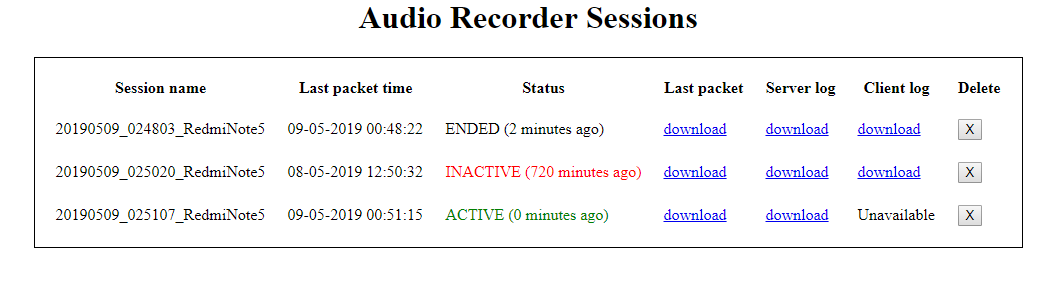
\includegraphics[width=1\textwidth]{obrazky-figures/dashboard.png}
	\caption{Dashbaord servera, ktorý zobrazuje všetky možné stavy session.}
	\label{dashboard}
\end{figure}


\subsection*{Spracovanie požiadaviek}

Už v popise protokolu v sekcii~\ref{protokol} boli predostreté typy požiadaviek, ktoré sa v rámci komunikácie klienta so serverom používajú. Následne bude vysvetlené, ako presne server na jednotlivé typy požiadaviek reaguje.

\begin{itemize}
\item {\textbf{Počiatočná požiadavka} značí nové pripojenie, server si teda identifikátor session musí uložiť do zoznamu rozpoznaných session. K záznamu si ukladá aj aktuálny čas, ako údaj k poslednej aktivite od daného pripojenia a jeho stav, ktorý je aktívny.}
\item {\textbf{Záznam do logu} nesúci konkrétnu správu sa vkladá do príslušného logovacieho súboru. Táto požiadavka nevyvoláva aktualizáciu poslednej aktivity, pretože nenesie segment.}
\item {\textbf{Segmenty} vyvolajú aktualizáciu poslednej aktivity, obsah sa pridá na koniec súboru s celou nahrávkou v rámci konkrétnej session a zároveň sa uloží do súboru, ktorý nesie posledný prijatý segment od danej session. Pre prípad strát sa kontroluje hodnota dĺžky záznamu v požiadavke, ktorá bola vypočítaná na strane klienta a porovnáva sa s tou vypočítanou na strane servera a pri nezhode to značí stratu časti záznamu. Server v takom prípade odosiela odpoveď s chybou, po ktorej si klient záznam ukladá a odošle opätovne.}
\item {\textbf{Ukončujúca požiadavka} značí zastavenie nahrávania a obsahuje klientský log. Server si pre danú session zmení jej stav z aktívneho na ukončený. Obsah klientského logu je uložený a sprístupnený v dashboarde. Ak by však prišli záznamy pre danú session aj po ukončení spojenia, stále ich ukladá (ošetrenie prípadu pre spomalenie internetového pripojenia, ktoré by malo za následok odoslanie požiadavky o ukončenie predtým, než sa stihne odoslať záznam).}
\end{itemize}

Server podporuje prijímanie a ukladanie logov a nahrávok aj zo sessions, ktoré nepozn. Nahrávania, ktoré prebehli bez účasti servera sa zo zariadenia odosielajú taktiež. Neprebehne tu nijaký handshake, ale prvá požiadavka je záznam do logu so špeciálnym označením. Pomocou neho sa vytvorí zložka pre session a pridá sa do zoznamu sessions. Ak server session už pozná, nič nové nevytvára, ale zároveň nenastaví stav session na aktívny. Ukladanie nahrávok a ukončenie odosielania prebieha štandardným spôsobom.

\begin{pagebreakavoid}
\subsection*{Štruktúra servera}

Hierarchia na serveri zabezpečuje jednoduchú orientáciu v nahrávkach a obsahoch logov. Na najvyššej úrovni sa nachádzajú PHP súbory pre riadenie servera, textový súbor so sessions a zložka, kde sa ukladajú nahrávky a logy. V nej má každá session samostatnú zložku, kde sa ukladajú všetky dáta s ňou spojené. Názorná ukážka hierarchie:

\dirtree{%
.1 server.php.
.1 index.php.
.1 sessions.txt.
.1 recordings.
.2 Timestamp1\_DeviceName.
.3 client.log.
.3 server.log.
.3 last\_packet.raw.
.3 recording.raw.
}
\end{pagebreakavoid}

\section{Testovanie}

Pri testovaní bolo hlavnou myšlienkou dokázať, že aplikácia je schopná nahrávať spoľahlivo a dlhodobo. Na overenie oboch týchto cieľových charakteristík som použila metódu nahrávania zvuku z generátora sínusového signálu\footnote{http://www.szynalski.com/tone-generator/} na 440 Hz. Pre prehrávanie a náhľad nahrávky bol použitý open source (otvorený zdrojový kód) multiplatformový editor zvuku Audacity\footnote{https://www.audacityteam.org/}. Hlbšia analýza signálu bola vykonaná pomocou programového prostredia MATLAB\footnote{https://www.mathworks.com/products/matlab.html}.

\subsection*{Náhľad nahrávky}

Po nahrávaní sínusového signálu s frekvenciou 440 Hz a nastavením frekvencie v aplikácii na  48 000 Hz a veľkosťou buffru 0.05 MB bol výsledkom záznam vo formáte RAW. Formát RAW je typický pre ukladanie nekomprimovaných audio dát a oproti ostatným formátom neobsahuje hlavičku s informáciami o frekvencii, bitovej hĺbke, endianite alebo konfigurácii kanálov. Pre prehrávanie RAW audio súborov je vyžadované manuálne zadanie týchto parametrov do programu, ktorý podporuje ich prehrávanie. Konkrétne Audacity ponúka možnosť importovať aj RAW audio a po nastavení jeho parametrov je možné ho prehrať. Po otvorení nahraného audia sa zobrazí nahrávka vo forme sínusového signálu, ako možno vidieť na obrázku~\ref{audacity_sinus_zoom}.


\begin{figure}[hbt]
	\centering
	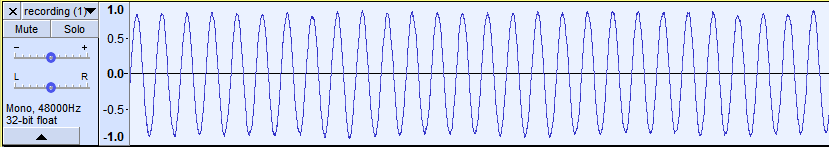
\includegraphics[width=1\textwidth]{obrazky-figures/audacity_sinus_zoom.png}
	\caption{Nahraný signál po zosilnení.}
	\label{audacity_sinus_zoom}
\end{figure}

Pri tejto metóde testovania bola zvolená menšia veľkosť buffru, aby sa dokázalo, že medzi jednotlivými segmentmi nebudú nijaké prerušenia alebo medzery, čo sa splnilo, keďže signál je súvislý celý svoj priebeh a po jeho prehraní je zvuková stopa plynulá a vierohodná.

\subsection*{Porovnanie nahraného a sínusového signálu}

Pre porovnanie týchto dvoch signálov bolo použité prostredie MATLAB, v ktorom bol najprv vykreslený krátky začiatočný segment nahraného signálu. Z dôvodu chýbajúcej podpory pre prácu s RAW formátom bol záznam konvertovaný do formátu WAV. Funkciou pre načítanie audio dát prebehne získanie vzoriek a frekvencie nahrávky. Následne sa vypočíta časová os, obmedzí sa rozsah celého signálu iba na krátky úsek z dôvodu prehľadnosti a vykreslí sa graf, ktorý reprezentuje vzorky zo zaznamenaného audia a je znázornený na obrázku~\ref{matlab_recorded}.


Pri vykresľovaní sínusovej funkcie, ktorá bola pôvodne nahrávaná je dôležité správne nastaviť posun a amplitúdu voči nahranému signálu, pretože hlasitosť pri nahrávaní zvyčajne nedosahuje krajných hodnôt a nahrávanie mohlo začať na ľubovoľnom mieste v rámci periódy. Po vypočítaní týchto konštánt sa môže originálny sínusový signál vykresliť k nahrávanému. Ako je z obrázku~\ref{matlab_comparison} zrejmé, signály sú si veľmi podobné. Avšak obrázok reprezentuje len malú časť nahrávky a je potrebné urobiť porovnanie na celom jeho rozsahu.

\begin{figure}[!hbt]
	\centering
	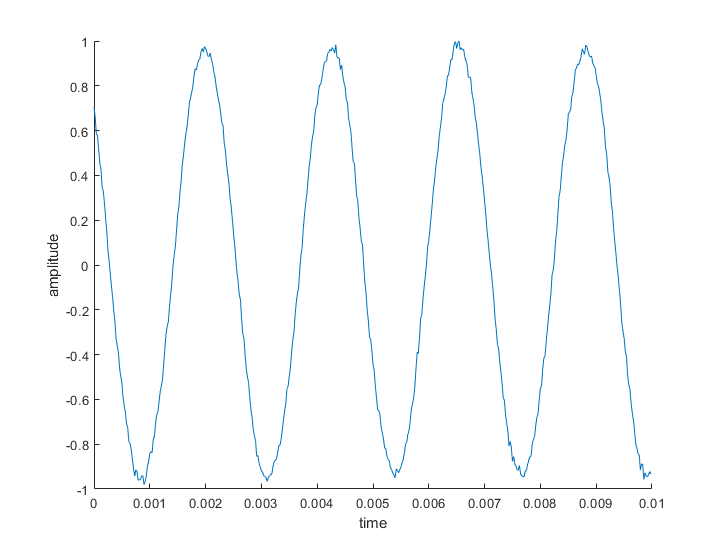
\includegraphics[width=0.9\textwidth]{obrazky-figures/matlab_recorded.png}
	\caption{Fragment nahraného signálu. Pri frekvencii 48 000 Hz je zobrazený priebeh amplitúdy o dĺžke 10 milisekúnd, čo zodpovedá 480 vzorkom.}
	\label{matlab_recorded}
\end{figure}

\begin{figure}[!hbt]
	\centering
	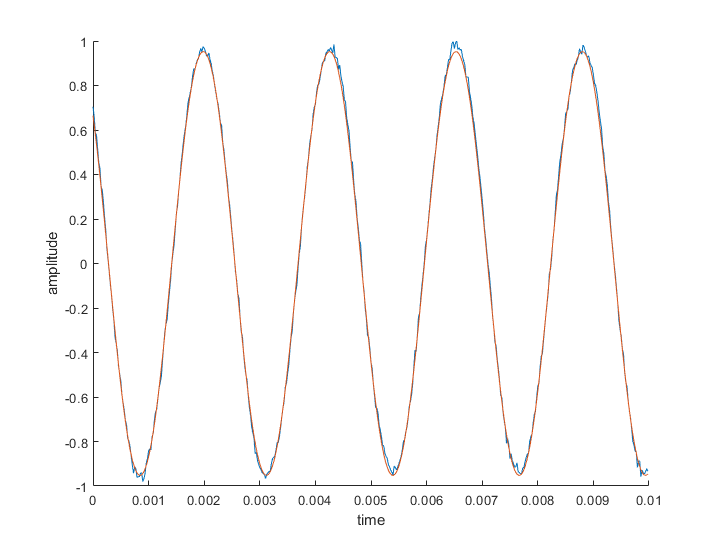
\includegraphics[width=0.9\textwidth]{obrazky-figures/matlab_comparison.png}
	\caption{Porovnanie nahraného a sínusového signálu. Nahraný signál je vykreslený modrou farbou a prekrýva ho oranžový sínusový signál.}
	\label{matlab_comparison}
\end{figure}


\FloatBarrier
\subsection*{Normalizovaná vzájomná korelácia signálov}

Vzájomná korelácia signálov je operácia, ktorá sa využíva ako meradlo podobnosti signálov. Môže byť použitá s jedným signálom (autokorelácia) alebo dvoma (korelácia). V praxi sa využíva najmä pri radarových alebo satelitných systémoch a pri poškodení signálu hlučnejším signálom.

V tomto prípade sa bude využívať vzájomná korelácia pre dva signály. Pre dva signály $x[k]$ a $y[k]$ je vzájomná korelácia definovaná prostredníctvom konvolúcie~\cite{Bracewell}.

\begin{equation}
	(x * y)[k] = \sum_{j=-{\infty}}^{\infty} x[j]y[j+k] \\
	\label{eq:eq1}
\end{equation}

Táto metóda však môže pre signály s rozdielnymi amplitúdami hlásiť vysoké podobnosti, preto je potrebné ju normalizovať~\cite{Bracewell}. Normalizovaná vzájomná korelácia je definovaná nasledovne:

\begin{equation}
	c(x, y)[k] = \frac{\sum_{j=-{\infty}}^{\infty} x[j]y[j+k]}{\sqrt{\sum_{j=-{\infty}}^{\infty} x^2[j]\sum_{j=-{\infty}}^{\infty} y^2[j+k]}} \\
	\label{eq:eq2}
\end{equation}

V prostredí MATLAB koreláciu sprostredkúva funkcia \texttt{xcorr()}\footnote{https://uk.mathworks.com/help/matlab/ref/xcorr.html}, ktorá po predaní parametru identifikujúceho normalizáciu vypočíta mieru podobnosti dvoch signálov. Pre výpočet je dôležitá maximálna absolútna podobnosť. Pre túto konkrétnu nahrávku vyšiel koeficient podobnosti 0,9986, čo potvrdzuje podobnosť signálov. Po dlhodobom nahrávaní sínusového signálu (5 hodín) v prostredí, kde sa v nahrávke vyskytovali zvuky z okolia mal koeficient nahrávky hodnotu 0,9621.

\subsection*{Delta signálov}

Koreláciou signálov sa dokázalo, že nahraný signál a sínusová funkcia sú takmer identické. Pomocou korelácie avšak nejde zistiť v ktorých bodoch nastali najväčšie odlišnosti a na základe toho skúmať prečo sa v daných bodoch nahraný signál líši od sínusového. 

Výpočtom rozdielu signálov (delta) sa signály porovnávajú v každom bode a ich funkčné hodnoty sa odčítajú. Tie vzniknuté hodnoty tvoria nový signál, ktorý predstavuje deltu nahraného signálu a sínusovej funkcie. Pri vysokej podobnosti signálov sa delta pohybuje okolo nulových hodnôt, pri výkyve v jednom zo signálov hodnota delty rastie. Delta signálov je znázornená na obrázku~\ref{delta}. 

\begin{figure}[!hbt]
	\centering
	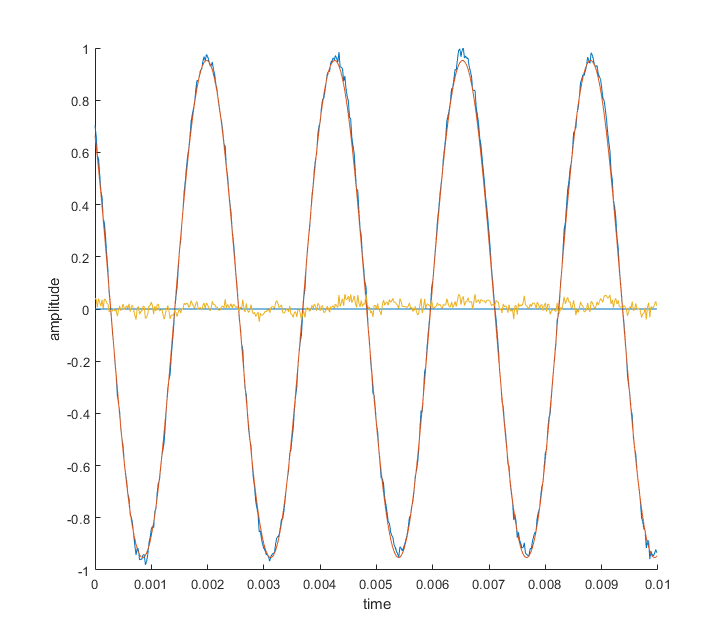
\includegraphics[width=0.9\textwidth]{obrazky-figures/delta.png}
	\caption{Delta nahraného a sínusového signálu. Delta predstavuje oranžový signál ktorého hodnoty sa nachádzajú okolo nuly. V strede je modrou farbou znázornený signál, ktorého hodnôt by delta nadobúdala, ak by boli signály úplne identické.}
	\label{delta}
\end{figure}

Pri testovaní s pomocou delty sa použili dva nahrávky, obe o dĺžke aspoň 5 hodín. Prvá nahrávka mala počas nahrávania v pozadí nežiadúce náhodné zvuky (rušenie), druhá bola nahrávaná v izolovanom tichom priestore. Obe nahrávky mali amplitúdu v rozsahu od -1 do 1 a po výpočte delty vznikli výsledky, ktoré sú uvedené v tabuľke~\ref{deltas}. Dôvodom vysokej maximálnej delty pri signále s rušením je náhle zvýšenie amplitúdy pri hlasných zvukoch. Príklad tohto javu je znázornený na obrázku~\ref{noise}.

\begin{table}[hbt]
\centering
\caption{Hodnoty delta funkcií v nahraných signáloch}
\label{deltas}
\begin{tabular}{|l|c|c|c|}
\hline
 & Minimum delty & Maximum delty & Priemerná delta  \\ \hline
Signál s rušením & 0,0028 & 3,1248 & 0,4043 \\ \hline
Signál bez rušenia & 0,0031 & 0,1094  & 0,0293 \\ \hline
\end{tabular}
\end{table}

\begin{figure}[!hbt]
	\centering
	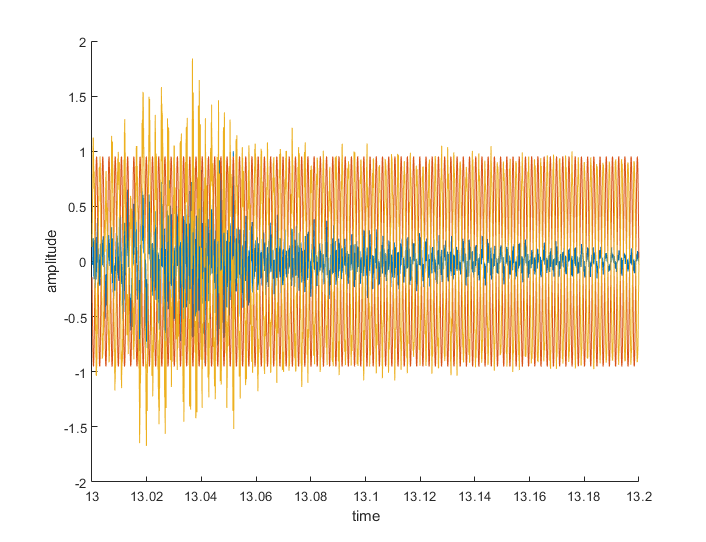
\includegraphics[width=0.9\textwidth]{obrazky-figures/noise.png}
	\caption{Ukážka rušenia v nahrávke. Modrou farbou je znázornená delta, ktorá sa v priebehu rušenia zväčšuje a neskôr sa opäť dostáva k nízkym hodnotám. Nahraný signál je označený žltou farbou a jeho zvýšená hlasitosť spôsobuje prečnievanie z intervalu amplitúdy daným sínusovým signálom.}
	\label{noise}
\end{figure}

\FloatBarrier
\pagebreak

\subsection*{Praktické testovanie}

Po vytvorení prvotnej verzie aplikácie a dobrých výsledkoch pri analýze nahrávania záznamov v radoch zopár hodín prebehlo praktické záťažové testovanie na viacero zariadeniach s trvaním v radoch desiatok hodín. Pri testovaní nebolo k dispozícii stabilné internetové pripojenie a aplikácia sa nachádzala na zariadeniach s ľubovoľnými verziami Androidu. Toto testovanie malo za úlohu dokázať že, aplikácia sa samovoľne nezrúti počas jej behu a že nestabilné internetové pripojenie nebude mať vplyv na jej fungovanie. Testovanie dokázalo spoľahlivosť aplikácie na zariadeniach, ktoré sú v uvedené v tabuľke~\ref{devices}.

\begin{table}[hbt]
\centering
\caption{Zariadenia, na ktorých prebehlo testovanie}
\label{devices}
\begin{tabular}{|c|c|}
\hline
Názov zariadenia & Verzia Androidu  \\ [0.5ex]
\hline\hline
Lenovo P70 & 4.4(KitKat)\\ \hline
LG L9 II (D605) & 4.4.2 (KitKat)\\ \hline
Asus Nexus 7 (2012) & 5.0 (Lollipop)\\ \hline
HTC One M8 & 6.0 (Marshmallow)\\ \hline
CAT S60 & 6.0.1 (Marshmallow) \\ \hline
Asus ZenPad 8.0 (P024) & 6.0.1 (Marshmallow)  \\ \hline
Samsung Galaxy S5 (SM-G900F) & 6.0.1 (Marshmallow) \\ \hline
Honor 8 (FRD-L09) &  7.0 (Nougat) \\ \hline
HTC One M9 & 7.0 (Nougat)\\ \hline
LG Nexus 5X  & 8.1 (Oreo)\\ \hline
Xiaomi Redmi Note 5 & 8.1 (Oreo)\\ \hline
\end{tabular}
\end{table}


\chapter{Záver}
\label{finale}

Cieľom tejto práce bola implementácia robustnej a spoľahlivej aplikácie pre nahrávanie reči na operačnom systéme Android, ktorá komunikuje so vzdialeným serverom a vyhovuje požiadavkám výskumu tak, aby predstavovala vhodný a použiteľný nástroj pri jeho vykonávaní. V súlade so skutočným stavom aplikácie a po testovaní bol cieľ teda splnený v plnom rozsahu.

V úvode práce je kladený dôraz na vysvetlenie funkcií aplikácie v rámci prípadu použitia a zdôvodnenie jednotlivých postupov. Nasleduje popis aktivít a procesov, na základe ktorých je zabezpečené spoľahlivé nahrávanie zvuku. V tejto časti sa nachádza prevažne len klientská časť, ktorá je detailne popísaná slovne, ale aj pomocou UML diagramov pre znázornenie súbežného behu viacero vlákien a toku udalostí pri kľúčových činnostiach ako napríklad nahrávanie a odosielanie. Tieto procesy sú charakteristické tým, že pracujú samostatne a za žiadnych okolností nijak neovplyvňujú samotné nahrávanie, čo je podstatou aplikácie. Pozornosť je venovaná aj konceptu nahrávania audia aj po stránke, ktorú automaticky vykonáva mobilné zariadenie, avšak jej pochopenie bolo dôležité pre vývoj aplikácie a vysvetlenie stavebných prvkov. Teória nahrávania audia je neoddeliteľnou súčasťou aplikácie aj kvôli tomu, že poskytuje vysvetlenie pre jednotlivé nastavenia, ktoré môžu ovplyvňovať vlastnosti audia a detailnejšie popisuje ich význam a použitie.

Časť popisujúca vývoj na Androide sa zameriava len na tie časti vývoja, ktoré priamo súvisia s aplikáciou. Pre prípad ďalšieho vývoja je popísaná štruktúra projektu. Aplikácia pracuje s istými komponentami Androidu, ktorých špecifické chovanie je popísané v tejto časti a obsahuje aj porovnania komponentov v rámci viacero verzií Androidu.

Implementácia sa delí na klientskú a serverovú. V klientskej je popísané primárne interné chovanie aplikácie, triedy a vzťahy medzi nimi, štruktúry a spôsoby cez ktoré sa audio dostane od zdroja až na server. Chybové a neočakávané stavy sú ošetrené s myšlienkou eliminácie strát audia. 

Serverová časť je výrazne menej obsiahla, keďže primárnou podstatou servera je len ukladať výstupy z procesov, ktoré prebiehajú v aplikácii a sú naň odoslané. Taktiež je v tejto časti popísané spôsob, akým server spravuje jednotlivé nahrávania a ako poskytuje prehľad o nahrávaní aj externe, bez potreby kontroly jednotlivých zariadení priamo.

Súčasťou implementačnej časti je aj testovanie, kde sa v dlhodobých časových intervaloch testovala funkcionalita aplikácie a servera. Simulovali sa aj rôzne nečakané stavy a analyzovala sa úplnosť a celistvosť výslednej nahrávky. 

\section{Ďalší vývoj}

Aplikácia je ľahko rozšíriteľná pre ďalšiu funkcionalitu týkajúcu sa manipulácie so zvukom. Dôležité je podotknúť, že momentálne je jej zameranie len v rámci výskumu, pre ktorý je určená a nie je určená pre širokú verejnosť. 

V serverovej časti by mohli pribudnúť prvky pre ľahšiu a prehľadnejšiu manipuláciu s jednotlivými sessions a to napríklad možnosť zmazania session aj so všetkými jej dátami, uvedenie konfigurácie audia pri nahrávaní, filtrovanie a vyhľadávanie v zozname sessions. Dashboard je statického charakteru a neaktualizuje sa v reálnom čase. Pri publikovaní aplikácie by bolo vhodné, aby sa do dashboardu pridala funkcia automatickej aktualizácie dát, napríklad pomocou technológie AJAX (asynchrónny JavaScript a XML). 

Do klientskej časti by mohla pribudnúť kompresia zvuku s detailným nastavením pre typ použitia, kde užívateľ nemá k dispozícii obsiahle úložisko a potrebuje nahrať dlhodobý záznam. Pribudnúť by mohla aj možnosť prehrávania záznamu skomponovaného na zariadení bez prítomnosti servera alebo všeobecne možnosť prehrania akéhokoľvek úseku audia. Toto momentálne nie je možné na väčšine štandardných mobilných audio prehrávačoch, pretože audio sa nahráva do formátu, ktorý neobsahuje hlavičku s informáciami o vzorkovacej frekvencii, bitovej hĺbke alebo nastavení kanálov. Prehliadanie úložiska zariadenia sa spolieha na zabudovaný prehliadač zložiek alebo externý. V prípade absencie prehliadača zložiek ponúka momentálne aplikácia manuálne zadanie cesty, avšak bolo by vhodnejšie napísať vlastný prehliadač zložiek, aby bolo prehliadanie zložiek prístupné aj na zariadeniach, ktoré ho nemajú nainštalovaný.

Spracovanie a manipulácia so zvukom je široká oblasť, ktorá sa len ťažko vyčerpá a do aplikácie by mohlo v budúcnosti pribudnúť veľa funkcií, ktoré by boli využiteľné v rámci širokej verejnosti.


%===============================================================================
